\documentclass[a4paper,12pt]{article}

% Paquetes básicos
\usepackage[utf8]{inputenc}
\usepackage[T1]{fontenc}
\usepackage[spanish]{babel}
\usepackage{graphicx}
\usepackage{xcolor}
\usepackage{lipsum}
\usepackage{geometry}
\geometry{top=3cm, bottom=3cm, left=2.5cm, right=2.5cm}

% Paquetes para diseño
\usepackage{titlesec}
\usepackage{fancyhdr}
\usepackage{amsmath}
\usepackage{amssymb}
\usepackage{hyperref}

% Paquetes para el entorno lstlisting
\usepackage{listings}
\usepackage{inconsolata}

%encabezado y pie de página nivel profesional
\usepackage{fancyhdr}
\pagestyle{fancy}
\fancyhf{}
\fancyhead[L]{\leftmark}
\fancyhead[R]{\rightmark}
\fancyfoot[L]{\textbf{Ismael Sallami Moreno - GIIADE}}
\fancyfoot[C]{\thepage}
\fancyfoot[R]{\textbf{(UGR)} \today}
\renewcommand{\headrulewidth}{0.4pt}
\renewcommand{\footrulewidth}{0.4pt}
\setlength{\headheight}{15pt}
\setlength{\headsep}{10pt}
\setlength{\footskip}{20pt}
\usepackage{truncate}
\fancyhead[L]{\truncate{0.5\headwidth}{\leftmark}}
\fancyhead[R]{\truncate{0.5\headwidth}{\rightmark}}
\usepackage{mathpazo}
\usepackage{tcolorbox}


% Paquete para fondo
\usepackage{background}
\usepackage{float}

% Configuración de lstlisting
\lstset{
    inputencoding=utf8,          % Permite UTF-8
    extendedchars=true,          % Reconoce caracteres extendidos
    literate=                    % Configuración manual para tildes y símbolos
        {á}{{\'a}}1
        {é}{{\'e}}1
        {í}{{\'i}}1
        {ó}{{\'o}}1
        {ú}{{\'u}}1
        {ñ}{{\~n}}1
        {Á}{{\'A}}1
        {É}{{\'E}}1
        {Í}{{\'I}}1
        {Ó}{{\'O}}1
        {Ú}{{\'U}}1
        {Ñ}{{\~N}}1
        {¿}{{\textquestiondown}}1
        {¡}{{\textexclamdown}}1,
    basicstyle=\ttfamily,        % Fuente monoespaciada
    breaklines=true,             % Habilita salto de línea automático
    frame=single,                % Marco alrededor del código
    backgroundcolor=\color{gray!10}, % Fondo gris claro
    keywordstyle=\color{blue},   % Color para palabras clave
    commentstyle=\color{green},  % Color para comentarios
    stringstyle=\color{red}      % Color para strings
}
\lstdefinestyle{customcpp}{
    language=C++,                % Lenguaje de programación
    showspaces=false,            % No mostrar espacios
    showtabs=false,              % No mostrar tabulaciones
    tabsize=4,                   % Tamaño de tabulación
    showstringspaces=false,      % No mostrar espacios en strings
    numbers=left,                % Números de línea a la izquierda
    numberstyle=\tiny\color{gray}, % Estilo de los números de línea
    numbersep=5pt,               % Separación de los números de línea
    stepnumber=1,                % Mostrar número en cada línea
    basicstyle=\ttfamily\footnotesize, % Estilo básico del código
    keywordstyle=\bfseries\color{blue}, % Estilo de las palabras clave
    commentstyle=\itshape\color{green!50!black}, % Estilo de los comentarios
    stringstyle=\color{red},     % Estilo de los strings
    identifierstyle=\color{black}, % Estilo de los identificadores
    % procnamekeys={def,class},    % Palabras clave para nombres de funciones
    morekeywords={constexpr,nullptr,size_t}, % Más palabras clave
    emph={int,char,double,float,unsigned}, % Palabras a enfatizar
    emphstyle=\color{magenta},   % Estilo de las palabras enfatizadas
    backgroundcolor=\color{gray!10}, % Color de fondo
    frame=shadowbox,             % Marco con sombra
    rulesepcolor=\color{gray},   % Color de la línea de separación
    breakatwhitespace=false,     % No cortar en espacios en blanco
    breaklines=true,             % Cortar líneas largas
    captionpos=b,                % Posición del título (abajo)
    escapeinside={(*@}{@*)},     % Delimitadores para escapar a LaTeX
    morecomment=[l][\color{magenta}]{\#}, % Comentarios de una línea
    morecomment=[s][\color{orange}]{/*}{*/}, % Comentarios multilínea
    morestring=[b]",             % Strings entre comillas dobles
    morestring=[b]'              % Strings entre comillas simples
}

% Configuración de título
\titleformat{\section}{\normalfont\Large\bfseries}{\thesection}{1em}{}

% Información del documento
\title{
    \vspace{-2cm}
    
\includegraphics[width=0.3\textwidth]{images/etsiit.png} \\ % Cambia el logo si es necesario
    \LARGE Ingeniería Informática + ADE\\
    \large Universidad de Granada (UGR)\\[1cm]
}
\author{\textbf{Autor:} Ismael Sallami Moreno}
\date{\textbf{Asignatura:} Tema 1 y Tema 2: Introducción y Capa de Red (FR)\\[1cm]}

% Configuración del fondo
\backgroundsetup{
    scale=1,
    color=black,
    opacity=0.2,
    angle=0,
    position=current page.south,
    vshift=0pt,
    hshift=0pt,
    contents={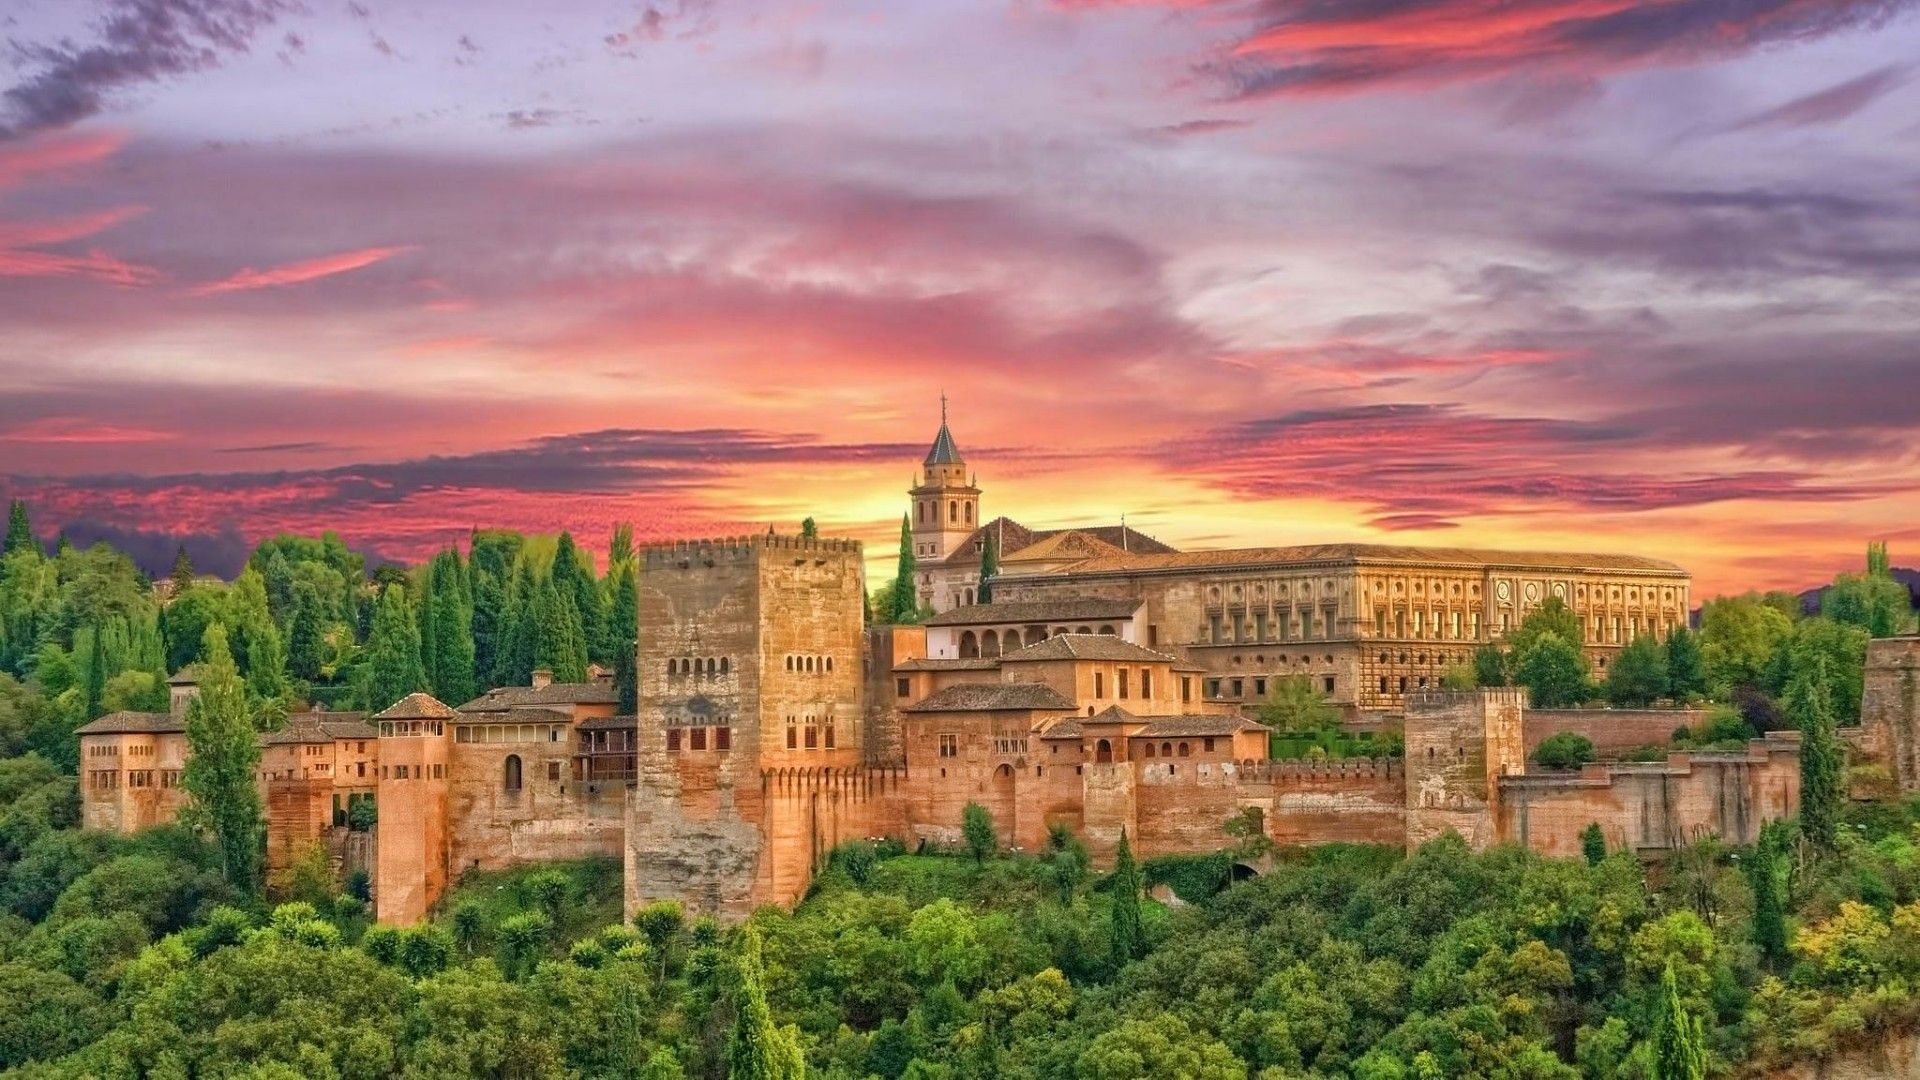
\includegraphics[width=\paperwidth,height=\paperheight,keepaspectratio]{images/granada.jpg}}
}

% Inicio del documento
\begin{document}

% Portada
\maketitle
\thispagestyle{empty}

\begin{center}
    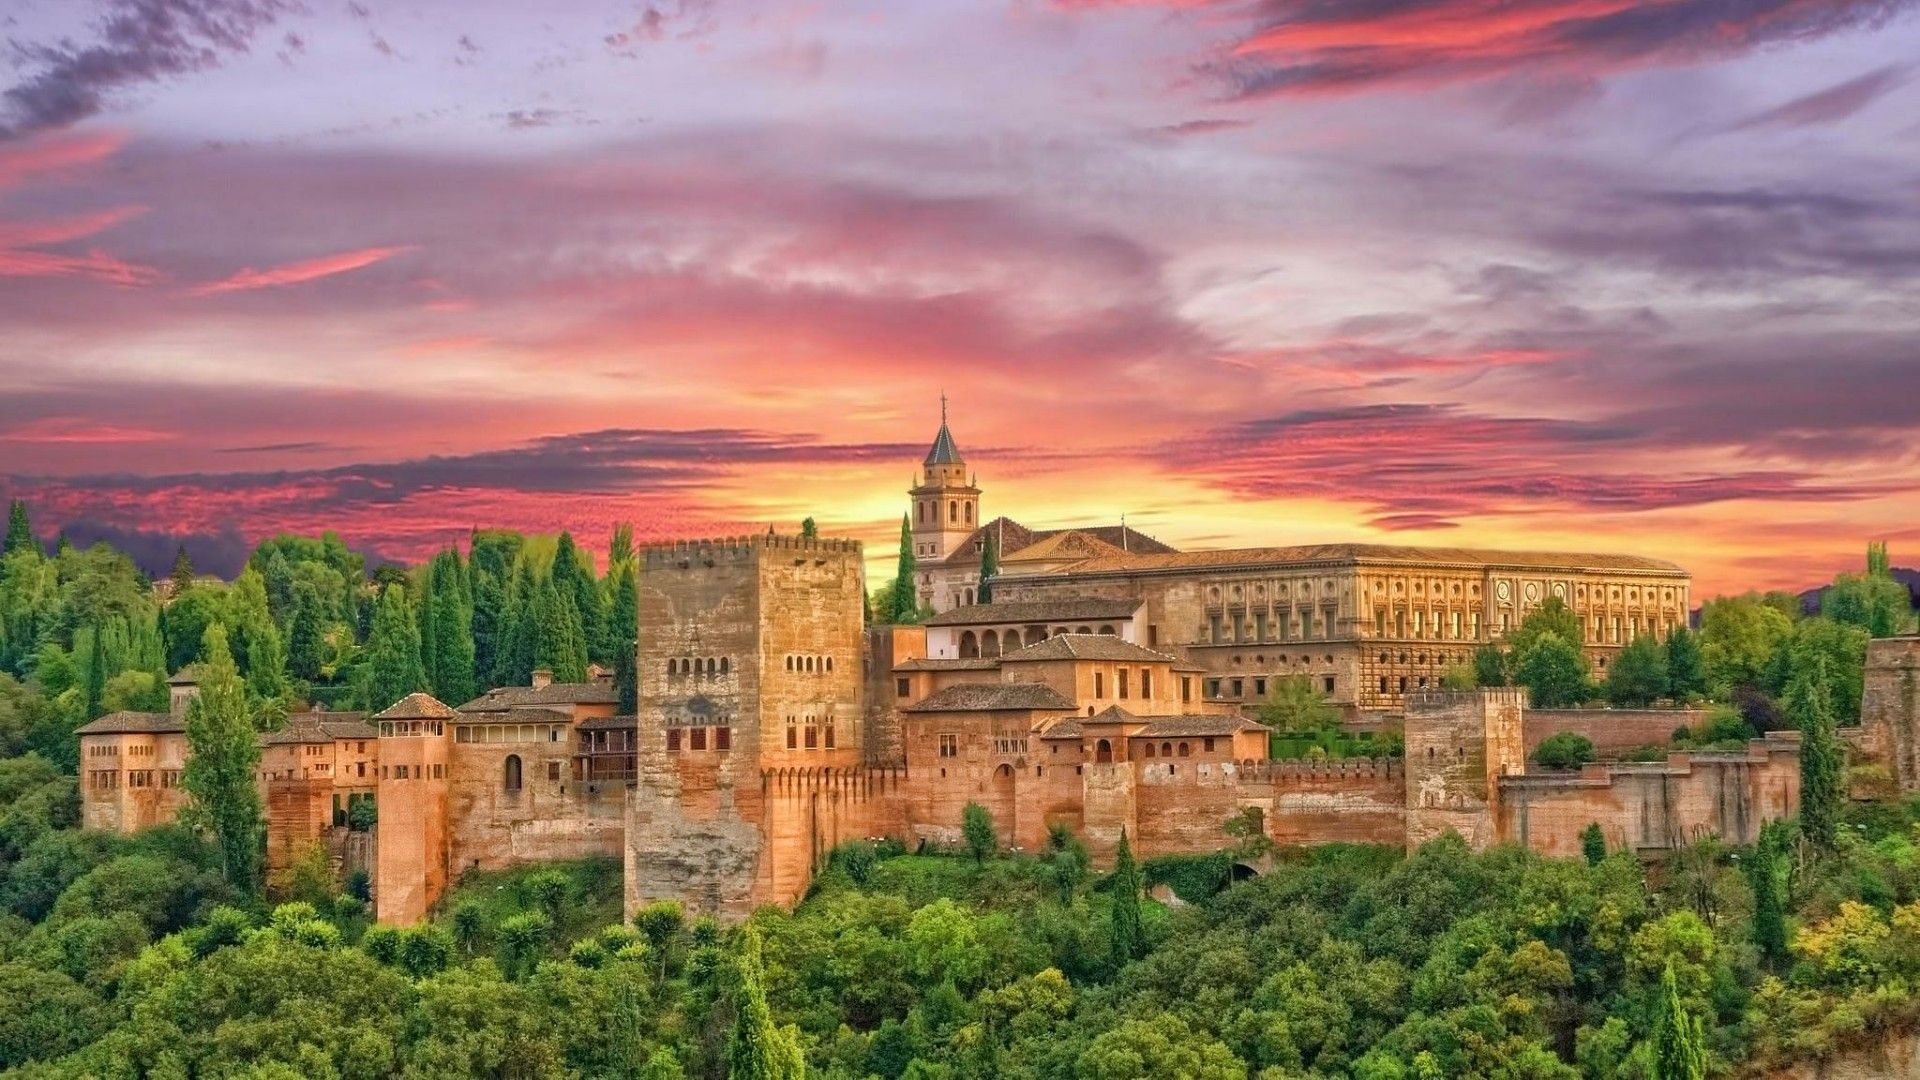
\includegraphics[width=\textwidth,height=0.4\textheight,keepaspectratio]{images/granada.jpg} \\ % Añade tu imagen de fondo
    \vfill
\end{center}

\newpage

% Índice (opcional)
\tableofcontents
\newpage

\textbf{Nota:}\textit{Se aconseja estudiar con ayuda de las diapositivas.}

\section{Tema 1: Introducción a los fundamentos de las redes}

\subsection{Sistemas de comunicación y redes}

Se define por un sistema de comunicación  a la infraestructura (hard y soft) que permite el intercambio de la información. La información es el conjuntos de datos que tienen un significado. Y por red entendemos al sistema de comunicación con sistemas finales y autónomos, que tiene capacidad de procesar la información. facilitando el intercambio eficaz y transparente de información.\\

La motivación para usar redes es la posibilidad de compartir recursos, la escalabilidad, fiabilidad, robustez, duplicidad y el ahorro de costes.\\

Características de una red, ya sea de computadores, de móviles, etc es la autonomía, la interconexión y el intercambio de información de manera eficaz y transparente.\\

Los elementos de una red son:
\begin{itemize}
    \item Hosts: sistemas finales, es decir, las terminales. Además son autónomos.
    \item Subred: es una infraestructura para el transporte de información. Esta consta de líneas de transmisión y nodos de elementos de comunicación, como pueden ser routers, switches, etc.
\end{itemize}

Ejemplos de medios de transmisión:
\begin{itemize}
    \item Cable coaxial
    \item Cable por trenzado: UTP, STP, FTP
    \item Fibra óptica
\end{itemize}

\subsubsection*{Topologías de redes: patrón de interconexión entre sus nodos}

\begin{itemize}
    \item Física vs lógica
    \item Tipos:
    \begin{itemize}
        \item En bus 
        \item En anillo
        \item En estrella
        \item En malla
        \item En árbol
        \item En híbrida
    \end{itemize}
\end{itemize}

\subsection{Clasificación de las redes}

\begin{itemize}
    \item Según su tamaño: PAN (personal), LAN(local), MAN(m3tropolitano), WAN(wide):
    \begin{itemize}
        \item PAN (Personal Area Network): Es una red utilizada para la comunicación entre dispositivos de una persona, típicamente en un rango de unos pocos metros. Ejemplos incluyen la conexión entre un teléfono móvil y un auricular Bluetooth.
        \item LAN (Local Area Network): Es una red que cubre un área geográfica pequeña, como una casa, oficina o edificio. Permite la interconexión de dispositivos como computadoras, impresoras y otros equipos dentro de un área limitada.
        \item MAN (Metropolitan Area Network): Es una red que abarca una ciudad o una gran área metropolitana. Se utiliza para conectar varias LANs dentro de una ciudad, proporcionando alta velocidad y conectividad eficiente.
        \item WAN (Wide Area Network): Es una red que cubre un área geográfica extensa, como un país o incluso continentes. Las WANs permiten la comunicación y el intercambio de datos entre dispositivos ubicados en diferentes lugares geográficos. Internet es el ejemplo más conocido de una WAN.
    \end{itemize}
    \item Según la tecnología de transmisión:
    \begin{itemize}
        \item Difusión: En este tipo de red, un solo nodo transmite datos a todos los demás nodos en la red. Un ejemplo común es la red de televisión por aire.
        \item Punto a punto: En este tipo de red, los datos se transmiten directamente entre dos nodos específicos. Un ejemplo común es una conexión telefónica.
    \end{itemize}
    \item Según el tipo de transferencia entre datos:
    \begin{itemize}
        \item \textbf{Simplex}: Es un modo de comunicación unidireccional, donde la información solo puede ser enviada en una dirección. Un ejemplo común es la transmisión de televisión.
        \item \textbf{Half-duplex}: Es un modo de comunicación bidireccional, pero no simultánea. Esto significa que la información puede ser enviada en ambas direcciones, pero no al mismo tiempo. Un ejemplo es un walkie-talkie.
        \item \textbf{Full-duplex}: Es un modo de comunicación bidireccional y simultánea. Esto significa que la información puede ser enviada y recibida al mismo tiempo. Un ejemplo es una llamada telefónica.
    \end{itemize}
\end{itemize}

\subsubsection{Nomenclatura típica en figuras}
    \begin{figure}[H]
        \centering
        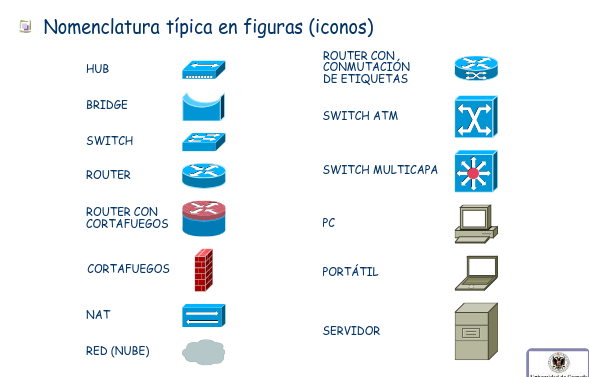
\includegraphics[width=0.8\textwidth]{images/nomenclatura.png}
    \end{figure}

\begin{itemize}
    \item \textbf{HUB}\footnote{Para la práctica, hay que saberse como mínimo HUB, SWITCH, ROUTER}: Dispositivo que conecta múltiples computadoras en una red local. Reenvía los datos recibidos a todos los dispositivos conectados.
    \item \textbf{ROUTER}: Encargado de dirigir paquetes de datos entre diferentes redes. Se utiliza para conectar redes locales a Internet o a otras redes.
    \item \textbf{SWITCH}: Dispositivo que conecta múltiples dispositivos en una red local, pero a diferencia de un HUB, envía los datos solo al dispositivo destinatario, mejorando la eficiencia.
    \item \textbf{BRIDGE}: Permite conectar dos redes locales separadas y filtrar el tráfico entre ellas en función de la dirección MAC.
    \item \textbf{SWITCH ATM}: Diseñado para redes que usan la tecnología de Modo de Transferencia Asíncrona (ATM), que transporta datos en celdas de longitud fija.
    \item \textbf{SWITCH MULTICAPA}: Similar a un switch, pero con la capacidad de operar en varias capas del modelo OSI, como la capa de red (3) y la capa de enlace (2).
    \item \textbf{ROUTER CON CORTAFUEGOS}: Combina las funciones de un router y un cortafuegos para proporcionar seguridad y dirigir tráfico en redes.
    \item \textbf{RED (NUBE)}: Representación abstracta de una red o conjunto de redes, que típicamente se utiliza para denotar servicios en la nube o conexiones externas.
    \item \textbf{NAT (Network Address Translation)}: Tecnología que permite que varios dispositivos compartan una única dirección IP pública mediante la traducción de direcciones.
    \item \textbf{PC}: Computadora personal que actúa como un host en una red.
    \item \textbf{SERVIDOR}: Computadora diseñada para proveer servicios a otros dispositivos en la red, como archivos, aplicaciones o datos.
    \item \textbf{PORTÁTIL}: Computadora portátil que también puede funcionar como host en una red.
    \item \textbf{CORTAFUEGOS}: Dispositivo o software diseñado para proteger redes bloqueando o permitiendo el tráfico en función de reglas predefinidas.
    \item \textbf{ROUTER CON CONMUTACIÓN DE ETIQUETAS}: Router que utiliza conmutación basada en etiquetas, como MPLS (Multiprotocol Label Switching), para optimizar el enrutamiento.
\end{itemize}

Los que debemos de saber dibujar son: \textbf{HUB, SWITCH, ROUTER.}

\subsubsection{Estructura y Elementos de una Red según Kurose y Ross}

La estructura y los elementos de una red están compuestos por diversos componentes que trabajan juntos para permitir la comunicación eficiente entre sistemas finales. Según Kurose y Ross, estos son los elementos principales:

\begin{itemize}
    \item \textbf{Hosts (Sistemas finales)}: 
    Dispositivos autónomos que actúan como origen o destino de la comunicación en una red. Los hosts pueden ser computadoras, servidores, dispositivos móviles o cualquier terminal que procese información.

    \item \textbf{Subred}: 
    La infraestructura que permite el transporte de información entre los sistemas finales. Dentro de una subred, encontramos dos elementos clave:
    \begin{itemize}
        \item \textbf{Líneas de transmisión}: Canales físicos o lógicos que transportan los datos entre los nodos de la red. Estos pueden ser cables de par trenzado, fibra óptica, enlaces inalámbricos, entre otros.
        \item \textbf{Nodos o elementos de conmutación}: Dispositivos intermedios como \textit{routers} o \textit{switches}, que se encargan de redirigir y gestionar el tráfico de datos dentro de la subred.
    \end{itemize}
\end{itemize}

Estos elementos se combinan para formar una red que facilita la interconexión y el intercambio de información de manera eficiente y transparente.

\subsection{Diseño y estandarización de redes}

Debemos de mencionar el \textit{Modelo de referencia} que engloba la definición de capas y de las funcionalidades. Para el diseño se deben de seguir ciertos apéndices:
\begin{itemize}
    \item Funcionalidades que son distintas deben de estar en capas distintas.
    \item Minimizar el flujo de información entre capas.
\end{itemize}

\subsubsection{Modelos OSI, TCP/IP y el concepto de RFC}

\subsubsection*{Modelos OSI y TCP/IP}

\begin{itemize}
    \item \textbf{OSI (Open Systems Interconnection)}: 
    Este modelo, desarrollado por la \textit{International Organization for Standardization (ISO)}, divide las comunicaciones de red en siete capas funcionales. Estas capas, que van desde la física hasta la aplicación, proporcionan un marco conceptual para la interoperabilidad entre sistemas.

    \item \textbf{TCP/IP (Transmission Control Protocol/Internet Protocol)}: 
    Es el modelo práctico utilizado para las comunicaciones en Internet, desarrollado por el \textit{Internet Engineering Task Force (IETF)}. Se compone de cuatro capas que se alinean funcionalmente con el modelo OSI.
\end{itemize}

\begin{figure}[H]
    \centering
    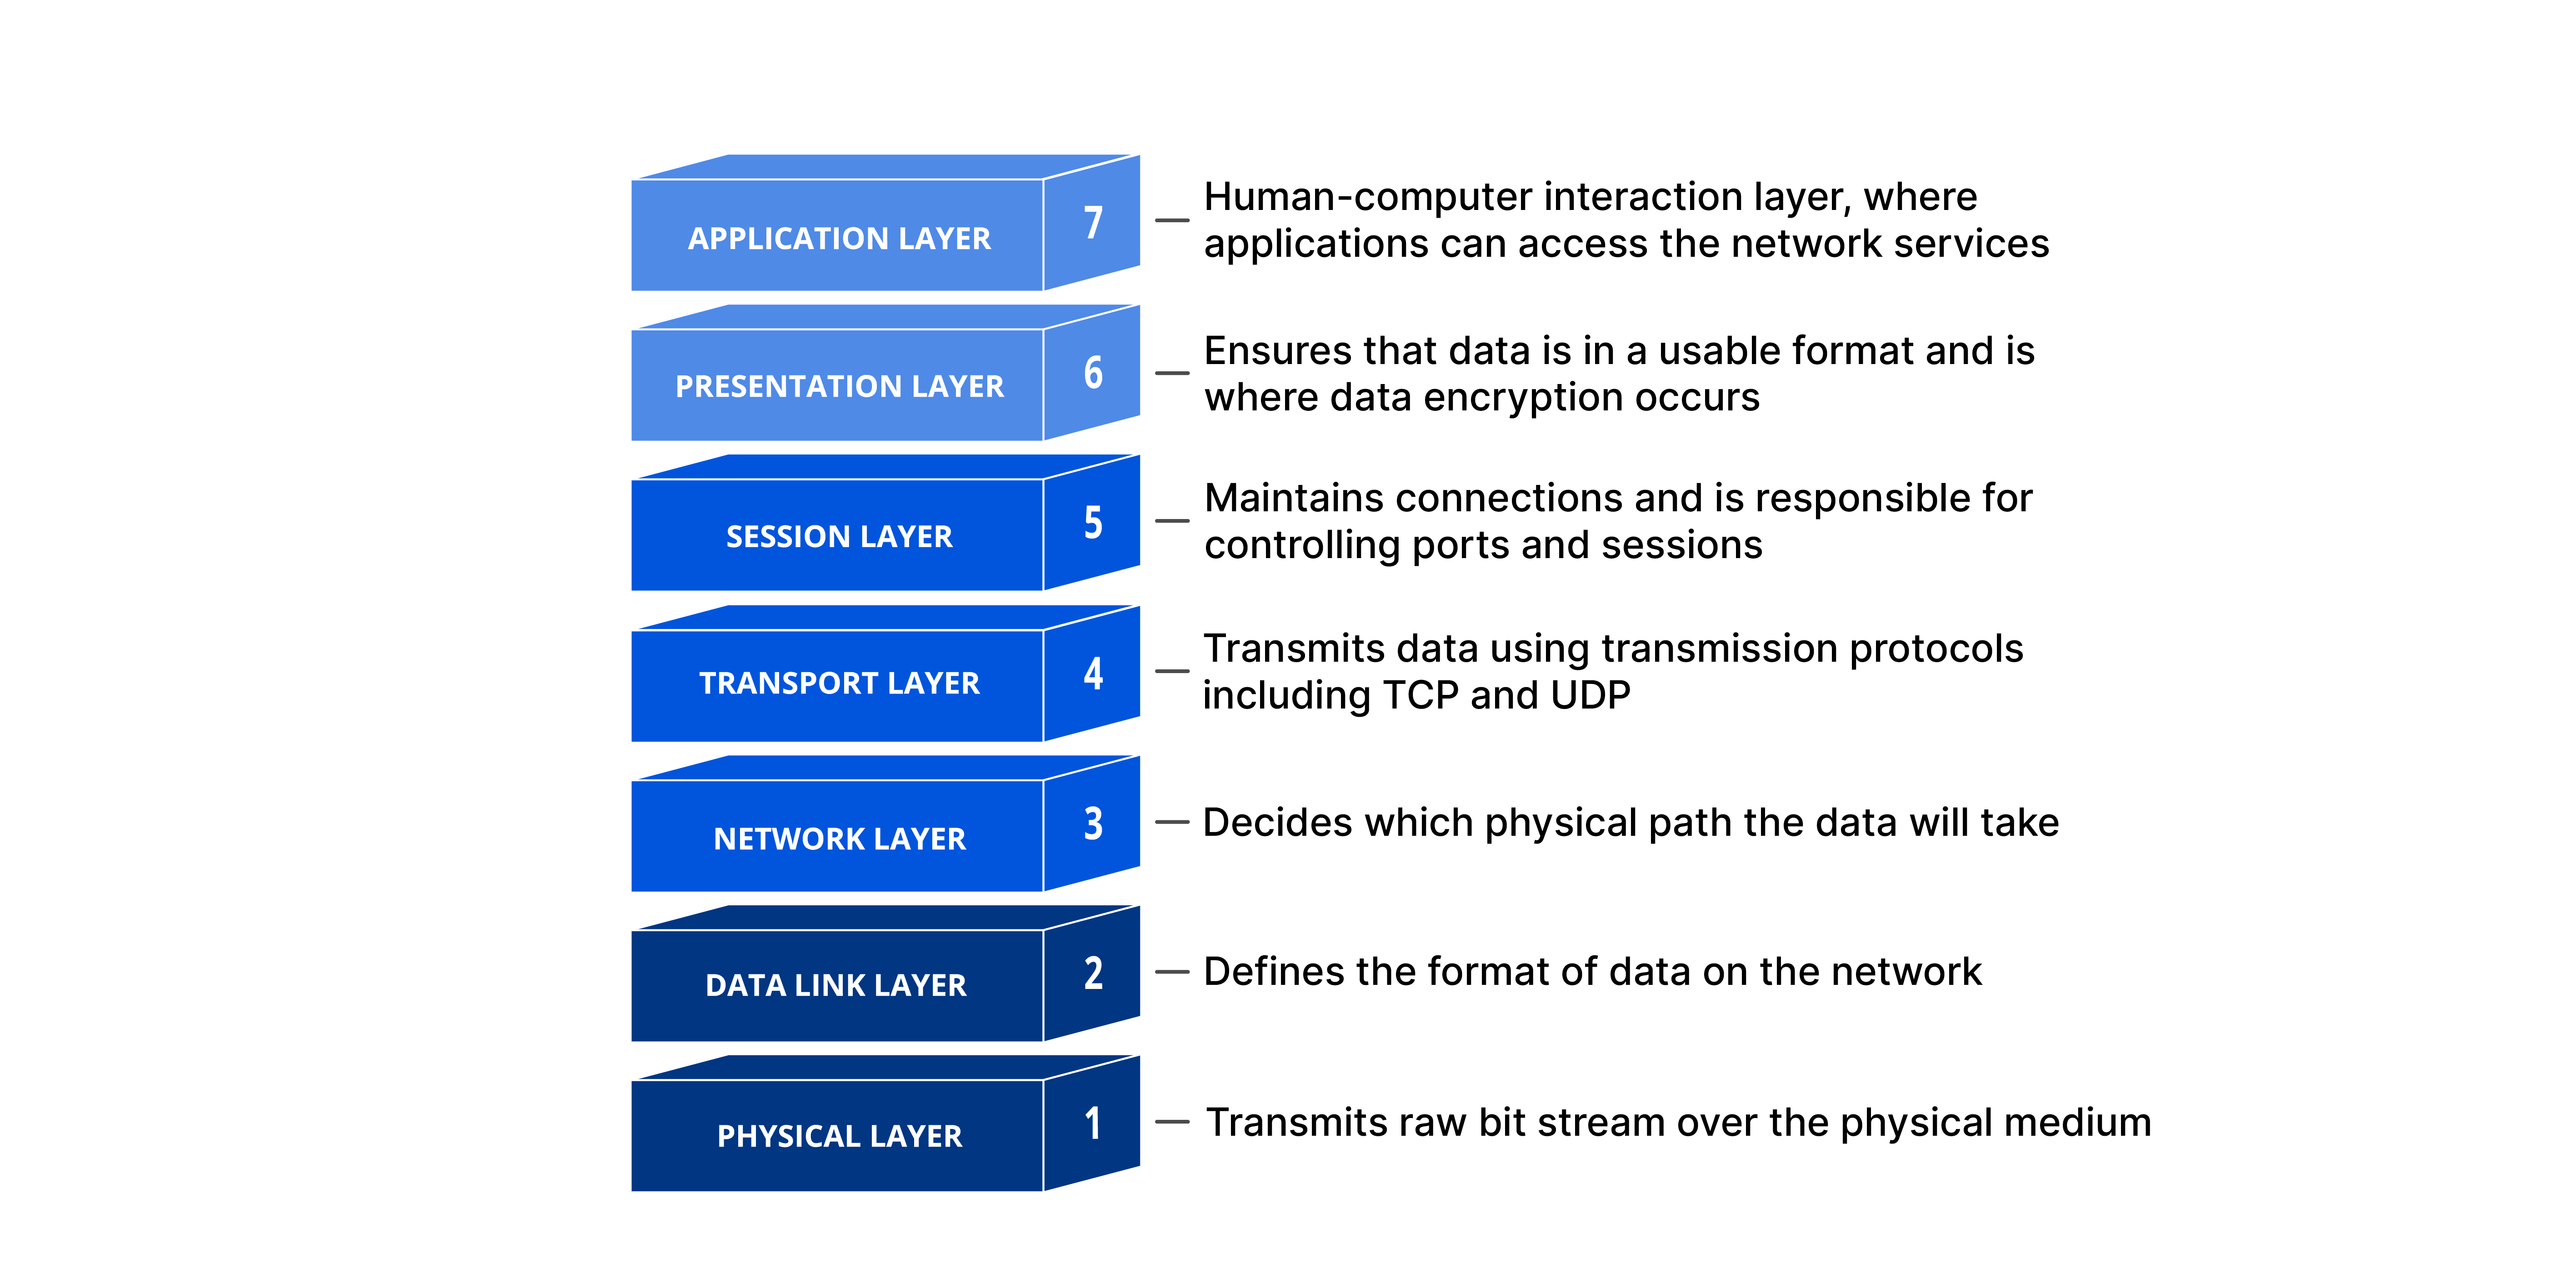
\includegraphics[width=0.8\textwidth]{images/osi.png}
    \hfill
    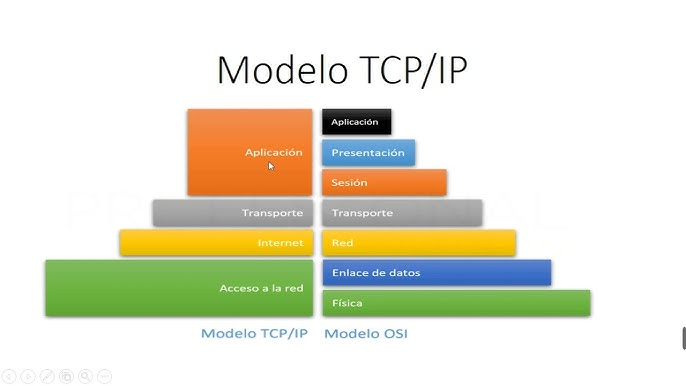
\includegraphics[width=0.8\textwidth]{images/TCP.jpg}
    \caption{Comparación entre el modelo OSI (arriba) y el modelo TCP/IP (abajo).}
    \label{fig:models}
\end{figure}

\subsubsection*{¿Qué es un RFC?}

El término \textbf{RFC (Request for Comments)} se refiere a una serie de documentos que contienen especificaciones, estándares y directrices sobre cómo funciona Internet y sus protocolos asociados. Estos documentos son gestionados por el \textit{RFC Editor} bajo la supervisión del \textit{Internet Engineering Task Force (IETF)}.

\begin{itemize}
    \item Los RFC pueden describir protocolos como HTTP, TCP, IP, entre otros.
    \item También incluyen métodos, tecnologías y recomendaciones para la evolución de la arquitectura de Internet.
\end{itemize}

Por ejemplo, el \textbf{RFC 2026} detalla el procedimiento de normalización para los estándares de Internet. Los RFC son esenciales para asegurar que dispositivos y sistemas de diferentes fabricantes puedan comunicarse de forma eficiente y uniforme.

\subsection{Terminología, conceptos y servicios}

\begin{figure}[H]
    \centering
    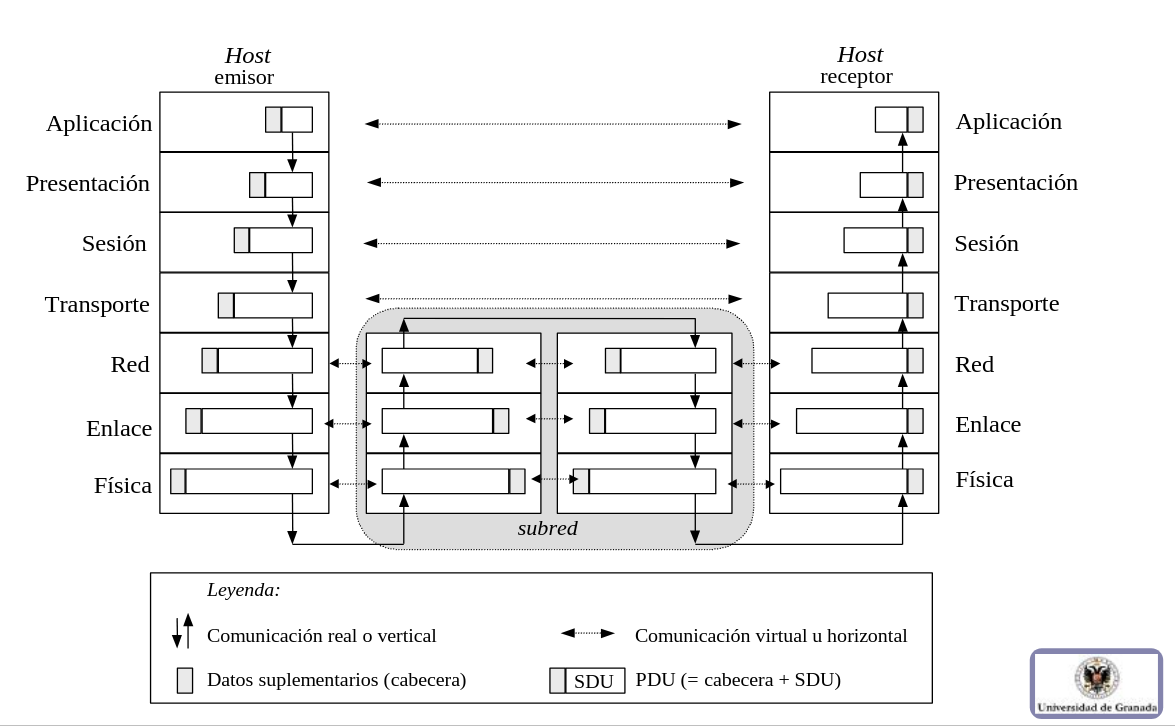
\includegraphics[width=1\textwidth]{images/osi_comparacion.png}
    \caption{Terminología y conceptos básicos en redes de computadoras.}
    \label{fig:terminology}
\end{figure}

\subsubsection*{Terminología, Conceptos y Servicios}

La terminología y los conceptos relacionados con las redes son esenciales para comprender cómo los dispositivos interactúan y cómo se estructuran las comunicaciones. A continuación, se detallan los términos principales:

\paragraph{Comunicación real (vertical):}
Es el intercambio de datos que ocurre entre capas adyacentes dentro de un dispositivo. Esta comunicación sigue un flujo descendente (del emisor) y ascendente (del receptor), en función del modelo de referencia utilizado.

\paragraph{Comunicación virtual (horizontal):}
Es la interacción lógica entre entidades pares en capas equivalentes de los dispositivos emisores y receptores. Aunque esta comunicación es conceptual, es facilitada por las capas inferiores.

\paragraph{Entidad del nivel N:}
Se refiere a una unidad funcional en la capa \(N\) del modelo OSI o similar. Por ejemplo, una entidad de la capa de transporte podría ser el protocolo TCP.

\paragraph{Entidades pares:}
Son entidades ubicadas en la misma capa de distintos dispositivos que se comunican mediante protocolos.

\paragraph{Protocolo:}
Es un conjunto de reglas que define cómo las entidades pares deben comunicarse. Incluye formatos, tiempos y secuencias de mensajes.

\paragraph{Interfaz:}
Es el punto de contacto entre capas adyacentes dentro de un dispositivo. Define cómo una capa accede a los servicios ofrecidos por la capa inferior.

\paragraph{Servicio:}
Es la funcionalidad que una capa provee a la capa superior. Por ejemplo, la capa de transporte ofrece servicios de entrega confiable a la capa de aplicación.

\paragraph{Capa proveedora y capa usuaria:}
La capa proveedora es aquella que ofrece un servicio, mientras que la capa usuaria lo consume. Por ejemplo, la capa de red es proveedora de la capa de transporte.

\paragraph{Pila de protocolos:}
Es la implementación de los protocolos en cada capa, que trabaja conjuntamente para permitir la comunicación de extremo a extremo.

\paragraph{Arquitectura de red:}
Es la combinación de un modelo de referencia (como OSI) y una pila de protocolos que define cómo funciona la red.

\paragraph{SAP (Service Access Point):}
Es un punto en la interfaz entre capas donde una capa accede a los servicios de otra. Se usa para identificar el punto de interacción.

\paragraph{SDU (Service Data Unit):}
Es la unidad de datos que una capa recibe de la capa superior para procesar y transmitir.

\paragraph{PDU (Protocol Data Unit):}
Es la unidad de datos intercambiada entre entidades pares en una capa. Incluye la SDU y cualquier información de encabezado o pie agregada por la capa.

\begin{figure}[H]
    \centering
    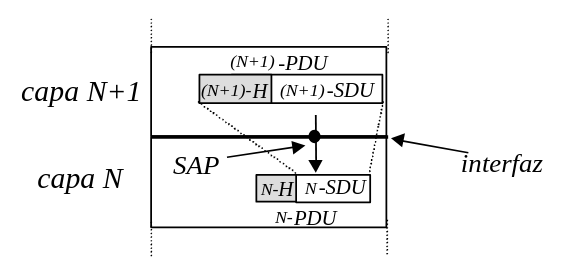
\includegraphics[width=0.5\textwidth]{images/capanycapanmas1.png}
\end{figure}

Estos conceptos son fundamentales para garantizar el \textit{intercambio de información transparente} entre los hosts, proporcionando una base sólida para entender cómo operan las redes modernas.

\subsubsection{Retardos en la comunicación}

\subsubsection*{Fórmulas}

Tiempo de transmisión:

\begin{equation}
    T_t = \frac{L}{V_t}
\end{equation}

Tiempo de propagación:

\begin{equation}
    T_p = \frac{D(m)}{V_t(m/s)}
\end{equation}

\begin{figure}[H]
    \centering
    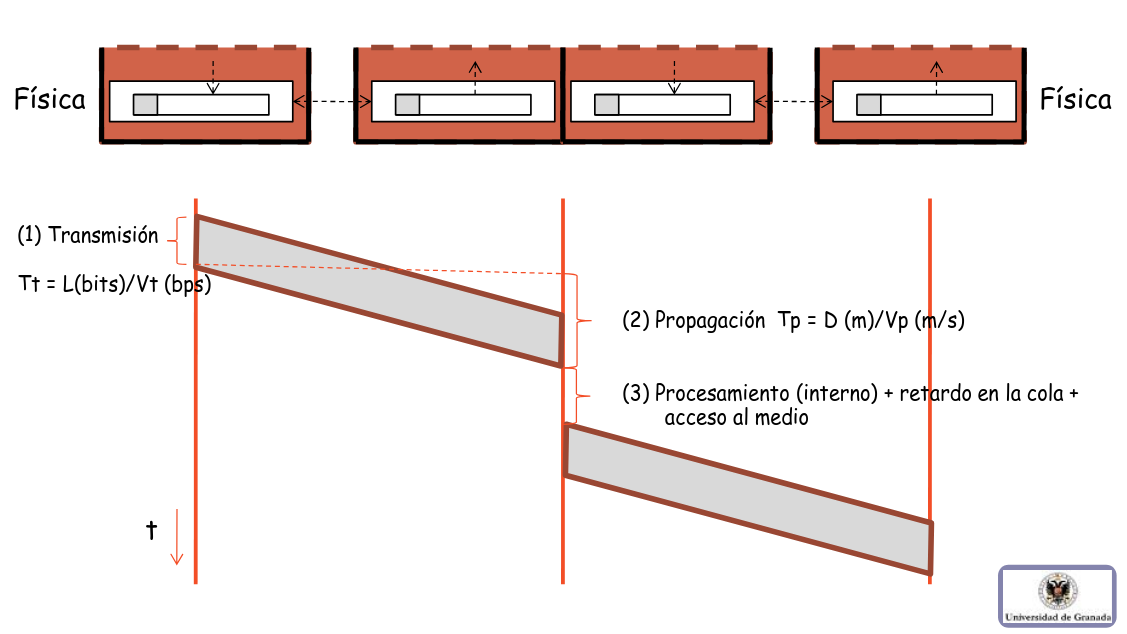
\includegraphics[width=0.8\textwidth]{images/RetardosComunicacions.png}
\end{figure}

%tcolorbox

\begin{tcolorbox}[colback=green!5!white, colframe=green!75!black, title=Nota]
    Si usamos la orden \textbf{ping} de una dirección, como por ejemplo de \textit{www.google.com}, podemos obtener el tiempo de ida y vuelta de los paquetes.
\end{tcolorbox}

\begin{tcolorbox}[colback=green!5!white, colframe=blue!75!black, title=Pregunta de Examen]
    \textbf{¿Qué es la congestión de red?} Podemos explicarlo mediante un caso práctico, como es, por ejemplo, mis routers tienen paquetes en cola, pues si salen pocos y entran muchos, descartan paquetes, y además conlleva que se reduzca la velocidad y por ende, se manden menos datos.   
    
\end{tcolorbox}

\subsubsection{Tipos de servicios}

\begin{itemize}
    \item Orientado a conexión (SOC): Se establece una conexión antes de enviar los datos.
    \item No orientado a conexión (SNOC): Se envían los datos sin establecer una conexión previa.
\end{itemize}

\begin{itemize}
    \item Confirmado (fiable): Se garantiza la entrega de los datos. Además, lleva un control de errores, de congestión, entrega ordenada.
    \item No confirmado (no fiable): No se garantiza la entrega de los datos.
\end{itemize}

\subsection{Internet: topología y direccionamiento}

Internet es una red global de redes interconectadas que permite la comunicación y el intercambio de información entre millones de dispositivos. Su diseño combina aspectos topológicos y de direccionamiento que aseguran su escalabilidad, eficiencia y robustez. A continuación, se resumen los aspectos clave:

\subsubsection{Topología de Internet}

La topología de Internet sigue una estructura jerárquica dividida en tres niveles principales:
\begin{itemize}
    \item \textbf{Intranets:} Redes privadas de los usuarios que incluyen tecnologías como Ethernet y WiFi. Estas redes están divididas en una zona pública y una zona privada para gestionar la seguridad y el acceso.
    \item \textbf{Redes de acceso:} Conectan a los usuarios finales con los Proveedores de Servicios de Internet (ISP). Algunos ejemplos de tecnologías utilizadas son xDSL, FTTH y RDSI.
    \item \textbf{Redes troncales:} Son infraestructuras de alta capacidad operadas por grandes proveedores de telecomunicaciones. Utilizan tecnologías como ATM, SDH, SONET o MPLS.
\end{itemize}

Además, los acuerdos entre estas redes, conocidos como \textit{peering} y conexiones de tránsito, permiten la comunicación entre operadores a nivel global. En este contexto, se diferencian las siguientes categorías:
\begin{itemize}
    \item \textbf{Redes Tier 1:} Operadores globales interconectados que forman el \textit{backbone} de Internet.
    \item \textbf{Redes Tier 2:} Operadores regionales que necesitan conectarse a redes Tier 1 para alcanzar toda Internet.
    \item \textbf{Redes Tier 3:} ISPs locales que proveen conectividad a usuarios finales y empresas.
\end{itemize}

\subsubsection{Direccionamiento en Internet}

\begin{figure}[H]
    \centering
    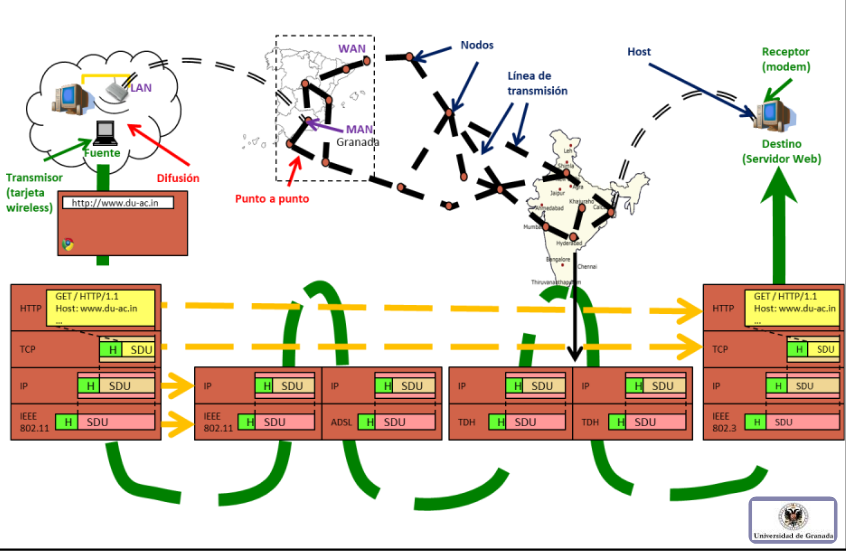
\includegraphics[width=0.8\textwidth]{images/internet.png}
    \caption{Estructura de Internet: topología y direccionamiento.}
    \label{fig:internet-topology-addressing}
\end{figure}


\subsubsection*{Explicación de la Imagen}

La imagen muestra una representación gráfica del tema ''Internet: topología y direccionamiento'' como parte de la introducción a los fundamentos de redes. Esta imagen es relevante porque ilustra cómo se estructura y se direcciona la información en una red de Internet, desde la fuente hasta el destino. A continuación, se detallan los elementos presentes en la imagen:

\begin{itemize}
    \item \textbf{Fuente y Transmisor}: La imagen comienza con una fuente de datos conectada a una red de área local (LAN) a través de un transmisor (tarjeta inalámbrica). Se muestra un ejemplo de una solicitud HTTP: \texttt{GET / HTTP/1.1 Host: www.dsc.uh.cu}.
    \item \textbf{Difusión y Punto a Punto}: La información se transmite desde la LAN a través de diferentes tipos de redes, incluyendo redes de área amplia (WAN) y redes de área metropolitana (MAN). Se destacan dos tipos de transmisión: difusión y punto a punto.
    \item \textbf{Nodos y Línea de Transmisión}: La información pasa a través de varios nodos y líneas de transmisión, representando la infraestructura física de Internet.
    \item \textbf{Receptor y Destino}: Finalmente, la información llega al receptor (modem) y al destino final, que es un servidor web. Se muestra otra solicitud HTTP similar a la inicial.
    \item \textbf{Capas del Modelo OSI}: La imagen también ilustra cómo los datos se encapsulan y desencapsulan a través de diferentes capas del modelo OSI (IEEE 802.11, IP, TCP, HTTP). Cada capa añade o quita su propio encabezado (H) y unidad de datos de servicio (SDU).
\end{itemize}

Esta imagen es interesante porque proporciona una visión clara y detallada de cómo se maneja y se dirige la información en una red de Internet, lo cual es fundamental para entender el funcionamiento de las redes de comunicación.


El direccionamiento en Internet se estructura en varios niveles, cada uno de los cuales cumple una función específica dentro de las diferentes capas del modelo TCP/IP:
\begin{itemize}
    \item \textbf{URL (Uniform Resource Locator):} Utilizado en la capa de aplicación para identificar recursos específicos, como páginas web. Ejemplo: \texttt{http://www.du-ac.in/index.html}.
    \item \textbf{Puertos:} Identifican los procesos de origen y destino en la capa de transporte. Por ejemplo, el puerto 80 para HTTP.
    \item \textbf{Dirección IP:} Se utiliza en la capa de red para identificar de manera única a los hosts en Internet.
\end{itemize}

% \begin{figure}[h!]
%     \centering
%     % Sustituir 'ruta_a_la_imagen.png' con la ruta de una imagen ilustrativa
%     \includegraphics[width=0.7\textwidth]{ruta_a_la_imagen.png}
%     \caption{Relación entre niveles de direccionamiento: URL, puertos y direcciones IP.}
%     \label{fig:direccionamiento}
% \end{figure}

\subsubsection{Otros elementos clave}

En Internet también se destacan los siguientes componentes:
\begin{itemize}
    \item \textbf{IXP (Internet Exchange Points):} Puntos de intercambio donde múltiples ISPs realizan \textit{peering}.
    \item \textbf{Red IRIS:} Ejemplo de una red académica y de investigación en España.
    \item \textbf{Redes autónomas:} Identificadas mediante ASNs (Autonomous System Numbers), que gestionan bloques de direcciones IP y políticas de enrutamiento.
\end{itemize}

Esta estructura asegura que Internet pueda soportar la enorme cantidad de tráfico generado por sus usuarios, garantizando conectividad global y optimización en el intercambio de datos.



\section{Tema 2: Capa de Red}

\subsection{Funcionalidades}

\subsubsection{Funciones y servicios en TCP/IP}
\begin{itemize}
    \item \textbf{Encaminamiento:} Proceso de seleccionar el camino más adecuado para enviar paquetes de datos desde el origen hasta el destino a través de una red. Ejemplo de protocolo: \textit{OSPF (Open Shortest Path First)}.
    \item \textbf{Conmutación:} Técnica utilizada para enviar datos a través de una red mediante la creación de una ruta temporal entre el origen y el destino. Ejemplo de protocolo: \textit{MPLS (Multiprotocol Label Switching)}.
    \item \textbf{Interconexión de redes:} Proceso de conectar diferentes redes para que puedan comunicarse entre sí, permitiendo el intercambio de datos. Ejemplo de protocolo: \textit{IP (Internet Protocol)}.
    \item \textbf{En OSI: control de gestión:} Función que supervisa y controla el funcionamiento de la red, asegurando que los recursos se utilicen de manera eficiente y que se mantenga la calidad del servicio. Ejemplo de protocolo: \textit{SNMP (Simple Network Management Protocol)}.
    \item \textbf{Ejemplos de protocolos de red:} Protocolos que operan en la capa de red para facilitar la comunicación entre dispositivos. Ejemplos incluyen \textit{IP (Internet Protocol)}, \textit{ICMP (Internet Control Message Protocol)}, y \textit{ARP (Address Resolution Protocol)}.
\end{itemize}

% \subsection{Conmutación}

% Es la acción de establecer o determinar un camino que permita transmitir la información de un punto a otro.

% \subsubsection*{Esquemas de conmutación}
% \begin{itemize}
%     \item Circuitos
%     \item Paquetes: datagramas o Circuitos virtuales
% \end{itemize}

\subsection{Conmutación}

La \textbf{conmutación} se refiere a la acción de establecer o determinar un camino que permita transmitir información de extremo a extremo en una red. A continuación, se describen los esquemas y conceptos principales asociados:

\subsubsection*{Esquemas de Conmutación}

Existen diferentes esquemas para implementar la conmutación en redes:
\begin{itemize}
    \item \textbf{Conmutación de Circuitos:} (Más adelante profundizaremos en este tema)
    \begin{itemize}
        \item Es un servicio orientado a conexión, lo que significa que requiere el establecimiento previo de una conexión antes de transmitir los datos.
        \item Ejemplo típico: redes telefónicas.
        \item Los pasos del proceso incluyen:
        \begin{enumerate}
            \item \textbf{Conexión:} Se establece un camino dedicado entre el emisor y el receptor.
            \item \textbf{Transmisión:} Los datos fluyen a través del circuito dedicado.
            \item \textbf{Desconexión:} El circuito se libera una vez finalizada la transmisión.
        \end{enumerate}
        \item Ventajas:
        \begin{itemize}
            \item Los recursos son dedicados, lo que facilita comunicaciones en tiempo real sin contención (es decir, sin competencia por el acceso al medio).
        \end{itemize}
        \item Inconvenientes:
        \begin{itemize}
            \item Retraso significativo para el establecimiento de la conexión.
            \item Baja flexibilidad para adaptarse a cambios en las condiciones de la red.
            \item Poco tolerante a fallos.
        \end{itemize}
    \end{itemize}

    \item \textbf{Conmutación de Paquetes:} (Más adelante profundizaremos en este tema)
    \begin{itemize}
        \item Utiliza datagramas o circuitos virtuales para transmitir información.
        \item En este esquema, los datos se dividen en paquetes pequeños, que se transmiten de forma independiente a través de la red.
        \item Ofrece mayor flexibilidad y tolerancia a fallos en comparación con la conmutación de circuitos.
    \end{itemize}
\end{itemize}

La elección entre conmutación de circuitos o de paquetes depende de las necesidades específicas de la red, como la prioridad de las comunicaciones en tiempo real frente a la adaptabilidad y tolerancia a fallos.

\subsubsection{Conmutación de Circuitos} 

La \textbf{conmutación de circuitos} es un esquema de transmisión que establece un camino fijo entre los dispositivos de origen y destino antes de que ocurra la comunicación. Este enfoque presenta varias ventajas y desventajas, las cuales se detallan a continuación:

\subsubsection*{Ventajas}

\begin{itemize}
    \item \textbf{Transmisión en tiempo real:} Ideal para servicios sensibles al tiempo, como la comunicación de voz.
    \item \textbf{Uso permanente de recursos:} Una vez establecido, el circuito permanece activo durante toda la sesión, garantizando estabilidad.
    \item \textbf{Sin contención:} No hay competencia por el acceso al medio, ya que los recursos están dedicados.
    \item \textbf{Circuito fijo:} La ruta de comunicación no cambia una vez configurada, eliminando decisiones de encaminamiento durante la transmisión.
    \item \textbf{Simplicidad en la gestión de nodos intermedios:} La operación de los nodos es más sencilla porque no necesitan reevaluar las rutas.
\end{itemize}

\subsubsection*{Desventajas}

\begin{itemize}
    \item \textbf{Retraso en el inicio de la comunicación:} Es necesario establecer el circuito antes de comenzar la transmisión, lo que genera un tiempo de espera.
    \item \textbf{Uso no eficiente de recursos:} Si el circuito permanece inactivo durante parte de la sesión, los recursos se desperdician.
    \item \textbf{Falta de flexibilidad:} El circuito es fijo y no se puede ajustar en caso de fallos o cambios en la red.
\end{itemize}

Este esquema es adecuado para aplicaciones donde la calidad de servicio y la baja latencia son esenciales, pero puede no ser ideal en escenarios donde la eficiencia en el uso de recursos es prioritaria.

\begin{figure}[H]
    \centering
    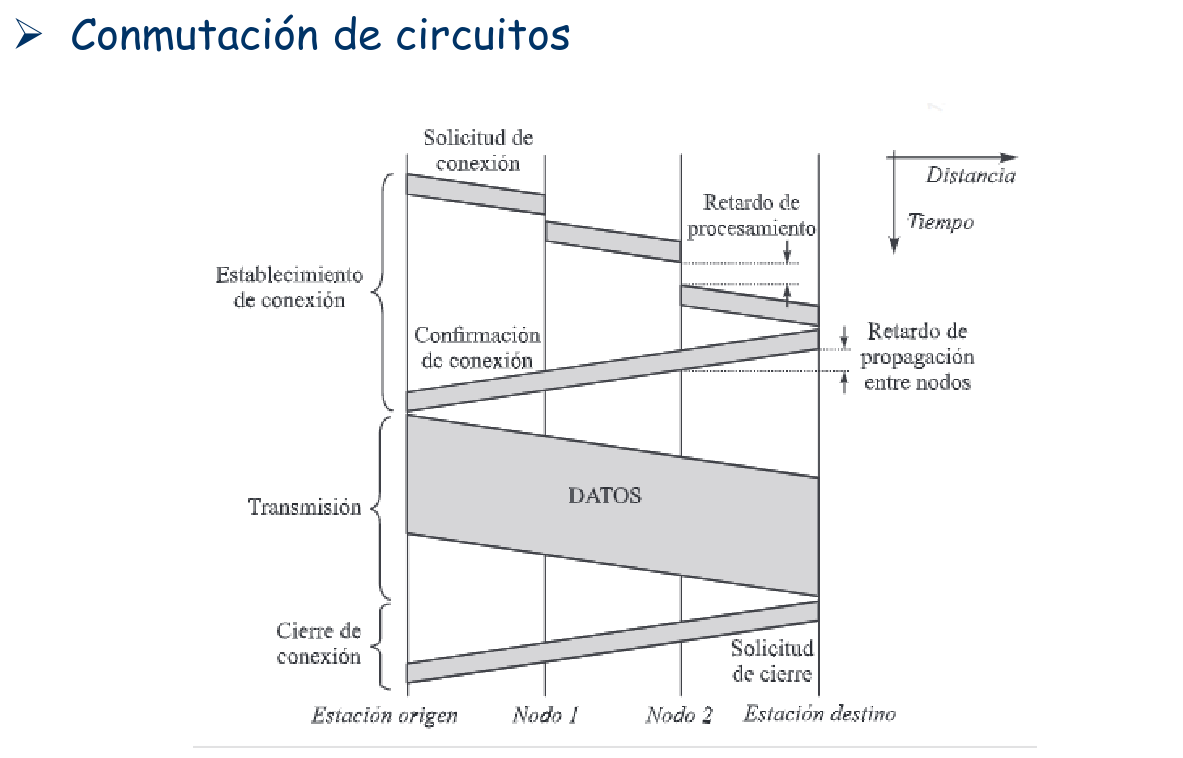
\includegraphics[width=0.9\textwidth]{images/conmutacionCircuitos.png}
    \caption{Ejemplo de conmutación de circuitos en una red telefónica.}
\end{figure}

\subsubsection{Conmutación de Paquetes}

La \textbf{conmutación de paquetes} es un esquema de transmisión en el que la información se divide en bloques denominados \textit{paquetes}. Estos paquetes se envían de manera independiente a través de la red, permitiendo flexibilidad y eficiencia en el uso de los recursos. 

\subsubsection*{Tipos de Conmutación de Paquetes}

\begin{itemize}
    \item \textbf{Conmutación mediante Datagramas:}
    \begin{itemize}
        \item Ejemplo: El protocolo IP.
        \item No requiere el establecimiento de una conexión previa.
        \item Los paquetes se envían de manera independiente, y cada uno puede seguir rutas diferentes a través de la red.
        \item En cada salto, los nodos intermedios realizan un proceso de \textit{almacenamiento y envío} (\textit{store-and-forward}), gestionando temporalmente los paquetes antes de retransmitirlos.
        \item Cada paquete contiene las direcciones de origen y destino, lo que permite que los nodos intermedios determinen su ruta.
    \end{itemize}
    
    \item \textbf{Conmutación de Paquetes con Circuitos Virtuales:}
    \begin{itemize}
        \item Ejemplo: ATM (\textit{Asynchronous Transfer Mode}), utilizado en redes troncales.
        \item Este esquema combina características de la conmutación de circuitos y de la conmutación de paquetes.
        \item Los pasos típicos incluyen:
        \begin{enumerate}
            \item \textbf{Conexión:} Se establece un circuito virtual antes de la transmisión.
            \item \textbf{Transmisión:} Los paquetes viajan a través del circuito virtual.
            \item \textbf{Desconexión:} El circuito virtual se libera al finalizar la transmisión.
        \end{enumerate}
        \item Los recursos no son dedicados, lo que permite mayor eficiencia en comparación con la conmutación de circuitos.
    \end{itemize}
\end{itemize}

\subsubsection*{Ventajas de la Conmutación de Paquetes}
\begin{itemize}
    \item Flexibilidad en la ruta de los paquetes, lo que incrementa la tolerancia a fallos en la red.
    \item Uso más eficiente de los recursos en comparación con la conmutación de circuitos.
    \item Adecuado para datos no sensibles al tiempo, como correos electrónicos y descargas de archivos.
\end{itemize}

\subsubsection*{Desventajas de la Conmutación de Paquetes}
\begin{itemize}
    \item Latencia variable debido a los posibles retrasos en los nodos intermedios.
    \item Requiere mayor capacidad de procesamiento en los nodos para almacenar y decidir el envío de los paquetes.
    \item Pérdida potencial de paquetes, lo que puede requerir retransmisión en aplicaciones críticas.
\end{itemize}

La conmutación de paquetes es el mecanismo predominante en redes modernas, especialmente en Internet, debido a su capacidad de manejar tráfico de datos heterogéneo y adaptarse dinámicamente a las condiciones de la red.


\subsubsection{Estimación del Tiempo de Transmisión en Conmutación de Paquetes mediante Datagramas}

La pregunta plantea estimar el tiempo total involucrado en la transmisión de un mensaje de datos utilizando la técnica de conmutación de paquetes mediante datagramas (\textbf{CDP}). Los parámetros proporcionados son:

\begin{itemize}
    \item \( M \): Longitud en bits del mensaje a enviar.
    \item \( V \): Velocidad de transmisión de las líneas en bits por segundo (\textit{bps}).
    \item \( P \): Longitud en bits de los paquetes.
    \item \( H \): Bits de cabecera de los paquetes.
    \item \( N \): Número de nodos intermedios entre las estaciones finales.
    \item \( D \): Tiempo de procesamiento en segundos en cada nodo.
    \item \( R \): Retardo de propagación en segundos asociado a cada enlace.
\end{itemize}

\subsubsection*{Solución Propuesta}

Para resolver el problema, debemos considerar:
\begin{enumerate}
    \item Dividir el mensaje en paquetes.
    \item Calcular el tiempo de transmisión por paquete.
    \item Incorporar los tiempos de procesamiento y propagación a lo largo de los nodos y enlaces.
\end{enumerate}

\paragraph{Cálculo del Tiempo Total de Transmisión}

\begin{align*}
    \text{Número de paquetes: } & \, N_p = \left\lceil \frac{M}{P - H} \right\rceil. \\
    \text{Tiempo de transmisión de un paquete: } & \, T_t = \frac{P}{V}. \\
    \text{Tiempo total de transmisión: } & \, T_{\text{total}} = N_p \cdot T_t + N_p \cdot N \cdot D + (N+1) \cdot R.
\end{align*}

Donde:
\begin{itemize}
    \item \( T_t \): Tiempo de transmisión de un paquete, calculado como el cociente entre el tamaño del paquete \( P \) y la velocidad de transmisión \( V \).
    \item \( T_{\text{total}} \): Tiempo total de transmisión, que incluye:
    \begin{itemize}
        \item La transmisión de todos los paquetes.
        \item El procesamiento en cada nodo (\( D \)).
        \item El retardo de propagación en los enlaces (\( R \)).
    \end{itemize}
\end{itemize}

\subsubsection*{Análisis de Validez de las Soluciones}

\paragraph{Solución Propuesta en las Diapositivas}
En el PDF\footnote{Como PDF se hace referencia a las diapositivas correspondientes al Temario 2, en específico, página 6/diapositiva 12} se menciona una fórmula similar basada en los mismos parámetros. La estructura general es válida, pero las diapositivas no siempre destacan la necesidad de sumar correctamente los retardos acumulados y los tiempos de procesamiento por cada paquete en nodos intermedios. Esto puede llevar a subestimar el tiempo total.

\paragraph{Solución Propuesta por ChatGPT}
La fórmula derivada en este documento, validada matemáticamente, considera cada paquete y su impacto en los tiempos de transmisión, procesamiento y propagación. Es válida y consistente con los principios de la conmutación de paquetes mediante datagramas.

\subsubsection*{Conclusión}

La solución propuesta aquí es válida, ya que incluye todos los retardos necesarios (transmisión, procesamiento y propagación) y maneja adecuadamente la fragmentación del mensaje en paquetes. 

Si las soluciones del PDF no consideran alguno de estos elementos, pueden estar incompletas. Sin embargo, las presentaciones del PDF son útiles como referencia siempre que se ajusten a los detalles planteados en este análisis.


\subsection{Protocolo IP}

\subsubsection{El Protocolo IP (IPv4)}

El protocolo IP versión 4 (\textbf{IPv4}), especificado en el RFC 791, es el estándar fundamental para la interconexión de redes, también conocidas como subredes. Sus principales características y funciones se describen a continuación:

\subsubsection*{Características de IPv4}

\begin{itemize}
    \item \textbf{Interconexión de redes:} IPv4 permite la comunicación entre diferentes subredes, resolviendo el problema del direccionamiento en Internet.
    \item \textbf{Retransmisión salto a salto:} Gestiona el envío de paquetes desde el host de origen al destino final a través de routers intermedios.
    \item \textbf{Servicio no orientado a conexión:}
    \begin{itemize}
        \item No realiza una negociación inicial o \textit{handshake}, lo que significa que no establece una conexión lógica entre los extremos.
        \item Es un protocolo \textit{no fiable}, ya que no implementa control de errores ni control de flujo.
    \end{itemize}
    \item \textbf{Unidad de datos:} Los paquetes enviados en IPv4 se denominan \textbf{datagramas}.
    \item \textbf{Protocolo de máximo esfuerzo (\textit{best-effort}):}
    \begin{itemize}
        \item No garantiza la entrega de los datagramas, que pueden perderse, duplicarse, retrasarse o llegar desordenados al destino.
    \end{itemize}
    \item \textbf{Gestión de fragmentación:} IPv4 adapta el tamaño de los datagramas a las diferentes \textit{Maximum Transfer Units} (MTUs) de las subredes, dividiendo los datagramas cuando es necesario.
\end{itemize}

\subsubsection*{Conclusión}

IPv4 es un protocolo básico y ampliamente utilizado en Internet. Aunque no garantiza la fiabilidad ni el orden de los datos transmitidos, su simplicidad y diseño permiten la interoperabilidad entre redes heterogéneas, lo que ha facilitado la expansión de la conectividad global.

\subsubsection*{Ejemplos}
\begin{itemize}
    \item Hotmail con servidor webmail 130.206.192.39
    \item Youtube \dots
    \item Google \dots
    \item Facebook \dots
\end{itemize}

\subsubsection*{Anotaciones Extra}

\begin{itemize}
    \item Las direcciones IP tienen 32 bits = 4 bytes
    \item No pueden ser mayores de 256  = 4 bytes
    \item Internet usa direccionamiento jerárquico, permitiendo clases, como la clase A, B, C, D, E, etc.
    \item Una de las máscaras que podemos tener es por ejemplo poniendo los 8 primeros bits a 1 y los 24 restantes a 0, es decir, 255.0.0.0
    \item ¿Que significa la red A?(podemos imaginar cualquier otra red). Pues significa que tenemos 128 redes de $2^{24} \approx 16$ millones.
    \item ¿Para que sirven las máscaras? Para ver la dirección IP que hay asociada a una red.
    
\end{itemize}

\subsubsection{Direccionamiento Jerárquico y Máscaras de Red en IPv4}

Internet adopta un esquema de \textbf{direccionamiento jerárquico} que simplifica el encaminamiento (\textit{routing}) al dividir las direcciones IP en dos partes claramente diferenciadas. Este sistema permite identificar subredes y dispositivos dentro de cada subred.

\subsubsection*{Estructura de las Direcciones IP}

Las direcciones IPv4 tienen un tamaño de \textbf{32 bits} y se dividen en dos componentes principales:
\begin{itemize}
    \item \textbf{Identificador de subred:} Representa la subred a la que pertenece el dispositivo.
    \item \textbf{Identificador de dispositivo (host):} Identifica de manera única al dispositivo dentro de la subred.
\end{itemize}

\subsubsection*{Máscaras de Red}

La \textbf{máscara de red} es un patrón que determina qué bits de una dirección IP corresponden al identificador de subred y cuáles al identificador del dispositivo. Se puede expresar de dos maneras:
\begin{itemize}
    \item \textbf{Notación decimal con puntos:} Ejemplo: \texttt{255.255.255.0}.
    \item \textbf{Notación CIDR (Classless Inter-Domain Routing):} Ejemplo: \texttt{200.27.4.112/24}, donde el número después de la barra indica la cantidad de bits asignados al identificador de subred.
\end{itemize}

\subsubsection*{Ejemplo de Cálculo del Identificador de Subred}

Dada una dirección IP y su máscara, el identificador de la subred se obtiene mediante una operación lógica AND:

\begin{verbatim}
Dirección IP:   200.27.4.112 = 11001000.00011011.00000100.01110000
Máscara:        255.255.255.0 = 11111111.11111111.11111111.00000000
------------------------------------------------------------------
Subred:         200.27.4.0   = 11001000.00011011.00000100.00000000
\end{verbatim}

\paragraph{Interpretación:}
\begin{itemize}
    \item \textbf{Dirección IP:} \texttt{200.27.4.112} identifica un dispositivo específico en la subred.
    \item \textbf{Máscara:} \texttt{255.255.255.0} indica que los primeros 24 bits (3 octetos) corresponden al identificador de subred.
    \item \textbf{Subred:} \texttt{200.27.4.0} es el identificador único de la subred a la que pertenece el dispositivo.
\end{itemize}

\subsubsection*{Ventajas del Direccionamiento Jerárquico}

\begin{itemize}
    \item \textbf{Simplificación del routing:} Reduce el tamaño de las tablas de encaminamiento al agrupar dispositivos en subredes.
    \item \textbf{Escalabilidad:} Permite gestionar redes de gran tamaño de manera eficiente.
    \item \textbf{Flexibilidad:} Las máscaras permiten subdividir redes en subredes más pequeñas para una asignación más granular de direcciones.
\end{itemize}

\subsubsection*{Conclusión}

El uso de direccionamiento jerárquico y máscaras de red es esencial para la organización eficiente de Internet y la gestión de sus recursos. Estos conceptos son fundamentales para comprender cómo se realiza el encaminamiento y la interconexión de dispositivos en redes modernas.

\subsubsection*{Internet}

Podemos considerar que Internet es un conjunto de subredes interconectadas. ¿Que es ... ?
\begin{itemize}
    \item \textbf{Una subred:} Es una subdivisión lógica de una red IP. Las subredes permiten segmentar una red más grande en redes más pequeñas, lo que facilita la gestión y mejora la eficiencia del uso de direcciones IP.
    \item \textbf{Un switch:} Es un dispositivo de red que conecta múltiples dispositivos dentro de una misma red local (LAN). Los switches operan en la capa de enlace de datos (capa 2 del modelo OSI) y utilizan direcciones MAC para enviar datos al dispositivo de destino correcto.
    \item \textbf{Un router:} Es un dispositivo de red que dirige paquetes de datos entre diferentes redes. Los routers operan en la capa de red (capa 3 del modelo OSI) y utilizan direcciones IP para determinar la mejor ruta para enviar los datos a su destino final.
\end{itemize}

Para determinar las subredes debemos de separar la interfaz de los hosts de los routers, creando redes aisladas, estas correspondes con las subredes.

\subsubsection*{¿Quién tiene las direcciones IP?}
Los hosts y los routers tienen 1 IP por cada interfaz, mientras que los switches no tienen direcciones.

\subsubsection{Elección de la Máscara de Red}

La elección de la máscara de red en una subred se basa en el número de dispositivos que se prevé alojar en dicha subred. Esto permite asignar direcciones IP de manera eficiente y evitar desperdiciar recursos.

\subsubsection*{Cálculo del Número de Dispositivos}

El número de direcciones disponibles para dispositivos en una subred se calcula utilizando la fórmula:
\[
\# \text{dispositivos} = 2^{\# \text{ceros en la máscara}} - 2
\]
\begin{itemize}
    \item El \(-2\) se debe a que la primera dirección (todos ceros) está reservada para identificar la subred y la última dirección (todos unos) está reservada para difusión (\textit{broadcast}).
    \item Por ejemplo, una máscara de \texttt{/24} (255.255.255.0) tiene 8 bits asignados al identificador de dispositivo, lo que permite \(2^8 - 2 = 254\) dispositivos.
\end{itemize}

\subsubsection*{Ejemplo Práctico}

Consideremos la dirección IP \texttt{200.27.4.112} con una máscara de red \texttt{255.255.255.0 (/24)}:
\begin{itemize}
    \item Dirección IP: \texttt{200.27.4.112} = \texttt{11001000.00011011.00000100.01110000}.
    \item Máscara: \texttt{255.255.255.0} = \texttt{11111111.11111111.11111111.00000000}.
    \item Subred: Realizando una operación lógica AND entre la dirección IP y la máscara, obtenemos:
    \begin{verbatim}
    Dirección IP:   200.27.4.112 = 11001000.00011011.00000100.01110000
    Máscara:        255.255.255.0 = 11111111.11111111.11111111.00000000
    ------------------------------------------------------------------
    Subred:         200.27.4.0   = 11001000.00011011.00000100.00000000
    \end{verbatim}
    \item Direcciones disponibles:
    \begin{itemize}
        \item \textbf{Reservada para subred:} \texttt{200.27.4.0}.
        \item \textbf{Primer dispositivo:} \texttt{200.27.4.1}.
        \item \textbf{Último dispositivo:} \texttt{200.27.4.254}.
        \item \textbf{Reservada para difusión:} \texttt{200.27.4.255}.
    \end{itemize}
\end{itemize}

\subsubsection*{Resumen del Ejemplo}

La máscara \texttt{/24} permite identificar una subred con hasta 254 dispositivos únicos. Este esquema asegura que cada subred tiene:
\begin{itemize}
    \item Un identificador único dentro de la red mayor.
    \item Direcciones reservadas para subred y difusión.
    \item Direcciones suficientes para todos los dispositivos necesarios.
\end{itemize}

\subsubsection*{Conclusión}

El uso de máscaras ajustadas al tamaño previsto de la subred optimiza la asignación de direcciones IP y facilita la gestión eficiente del espacio de direcciones disponible.


\subsubsection{Tipos de direcciones}
Para saber que es un \textit{Intranet} pincha \href{https://github.com/ElblogdeIsmael/ElblogdeIsmael.github.io/blob/main/Asignaturas/Tercer\%20A\%C3\%B1o/FR/Resumenes/ETSIIT/intranet.md}{aquí}.
\begin{itemize}
    \item Direcciones Públicas: cada dirección se asigna solo a un dispositivo en Internet y se asigna de manera centralizada.
    \item Direcciones Privadas: solo en intranets, se pueden repetir en distintas intranets. Las asigna el usuario según su criterio.
\end{itemize}

% \subsubsection{Direccione IP Clases}

% Los hosts y routers tienen 1 IP por cada una de sus interfaz

\subsubsection{Direcciones IP: Clases}

Las direcciones IP, según el estándar IPv4, tienen un tamaño de \textbf{32 bits} y se representan en \textit{notación decimal con puntos}. Cada dirección identifica un dispositivo o interfaz en una red. 

\subsubsection*{Aspectos generales de las direcciones IP}
\begin{itemize}
    \item Cada \textbf{host} o \textbf{router} tiene una dirección IP para cada una de sus interfaces de red.
    \item Las direcciones IP están organizadas en \textbf{5 clases principales}, descritas en el \textbf{RFC 1166}.
    \item La estructura de las clases determina la jerarquía y el uso de las direcciones:
    \begin{itemize}
        \item Clases \textbf{A}, \textbf{B}, y \textbf{C} son jerárquicas a dos niveles: \textit{identificador de red} + \textit{identificador de dispositivo}.
        \item Clases \textbf{D} y \textbf{E} tienen propósitos específicos (multidifusión y uso futuro, respectivamente).
    \end{itemize}
\end{itemize}

\subsubsection*{Descripción de las Clases}
\begin{itemize}
    \item \textbf{Clase A:}
    \begin{itemize}
        \item Primer bit: \(0\).
        \item Identificador de red: \(7\) bits.
        \item Identificador de host: \(24\) bits.
        \item Rango de direcciones: \(0.0.0.0\) a \(127.255.255.255\).
        \item Uso: Redes muy grandes, con muchas direcciones de host disponibles.
    \end{itemize}

    \item \textbf{Clase B:}
    \begin{itemize}
        \item Primeros dos bits: \(10\).
        \item Identificador de red: \(14\) bits.
        \item Identificador de host: \(16\) bits.
        \item Rango de direcciones: \(128.0.0.0\) a \(191.255.255.255\).
        \item Uso: Redes medianas a grandes.
    \end{itemize}

    \item \textbf{Clase C:}
    \begin{itemize}
        \item Primeros tres bits: \(110\).
        \item Identificador de red: \(21\) bits.
        \item Identificador de host: \(8\) bits.
        \item Rango de direcciones: \(192.0.0.0\) a \(223.255.255.255\).
        \item Uso: Redes pequeñas, con pocos dispositivos por red.
    \end{itemize}

    \item \textbf{Clase D:}
    \begin{itemize}
        \item Primeros cuatro bits: \(1110\).
        \item Rango de direcciones: \(224.0.0.0\) a \(239.255.255.255\).
        \item Uso: Multidifusión (\textit{multicast}).
    \end{itemize}

    \item \textbf{Clase E:}
    \begin{itemize}
        \item Primeros cinco bits: \(11110\).
        \item Rango de direcciones: \(240.0.0.0\) a \(255.255.255.255\).
        \item Uso: Reservadas para propósitos futuros.
    \end{itemize}
\end{itemize}

\subsubsection*{Ejemplo}
Una dirección IP en clase C, como \texttt{192.168.212.60}, tiene la siguiente estructura:
\begin{itemize}
    \item Identificador de red: \(192.168.212\).
    \item Identificador de host: \(60\).
\end{itemize}

% \subsubsection*{Conclusión}
% El esquema de clases de direcciones IP permite una organización jerárquica que facilita el \textit{routing} y la asignación eficiente de direcciones en redes de diferentes tamaños. Sin embargo, el modelo de clases ha sido reemplazado en gran medida por la notación \textbf{CIDR} (\textit{Classless Inter-Domain Routing}) en redes modernas.

Para ver detalladamente el cáculo de los rangos pincha \href{https://github.com/ElblogdeIsmael/ElblogdeIsmael.github.io/blob/main/Asignaturas/Tercer%20A%C3%B1o/FR/Resumenes/ETSIIT/rangosIPcalculo.md}{aquí}.

\subsubsection{Clases de Direcciones IP y Reglas Especiales}

Las direcciones IPv4 están organizadas en cinco clases principales (A, B, C, D y E) según su propósito y estructura. A continuación, se describen sus rangos, usos y reglas especiales.

\subsubsection*{Rangos y Capacidad por Clase}
\begin{itemize}
    \item \textbf{Clase A:}
    \begin{itemize}
        \item Rango: \texttt{0.0.0.0 – 127.255.255.255}.
        \item Redes disponibles: \(128\) redes.
        \item Capacidad: \(16,777,216\) hosts por red.
    \end{itemize}

    \item \textbf{Clase B:}
    \begin{itemize}
        \item Rango: \texttt{128.0.0.0 – 191.255.255.255}.
        \item Redes disponibles: \(16,384\) redes.
        \item Capacidad: \(65,536\) hosts por red.
    \end{itemize}

    \item \textbf{Clase C:}
    \begin{itemize}
        \item Rango: \texttt{192.0.0.0 – 223.255.255.255}.
        \item Redes disponibles: \(2,097,152\) redes.
        \item Capacidad: \(256\) hosts por red.
    \end{itemize}

    \item \textbf{Clase D:}
    \begin{itemize}
        \item Rango: \texttt{224.0.0.0 – 239.255.255.255}.
        \item Uso: Reservado para \textbf{multidifusión (multicast)}.
    \end{itemize}

    \item \textbf{Clase E:}
    \begin{itemize}
        \item Rango: \texttt{240.0.0.0 – 255.255.255.255}.
        \item Uso: Reservado para \textbf{fines futuros}.
    \end{itemize}
\end{itemize}

\subsubsection*{Reglas Especiales}
\begin{itemize}
    \item Direcciones con el identificador de host \(00\ldots0\): 
    \begin{itemize}
        \item Identifican una red.
        \item Nunca se usan como dirección de origen ni se asignan a dispositivos.
    \end{itemize}
    
    \item Direcciones con el identificador de host \(11\ldots1\):
    \begin{itemize}
        \item Se utilizan para difusión (\textbf{broadcast}) dentro de la red especificada.
        \item Nunca se asignan a dispositivos.
    \end{itemize}

    \item Dirección especial \texttt{127.0.0.0}:
    \begin{itemize}
        \item Reservada para pruebas de \textbf{autobucle (loopback)}.
        \item Utilizada para comprobar la configuración de red local.
    \end{itemize}
    
    \item Restricción adicional:
    \begin{itemize}
        \item Para evitar ambigüedades, el identificador de dispositivo no debe ser \(255\) ni \(0\).
    \end{itemize}
\end{itemize}

\subsubsection*{Direcciones IP Privadas (RFC 1918)}
El \textbf{RFC 1918} reserva rangos de direcciones IP para uso privado dentro de redes internas. Estas direcciones no se enrutan en Internet y se utilizan comúnmente en intranets.
\begin{itemize}
    \item \textbf{Clase A:} \texttt{10.0.0.0} – \(1\) red privada.
    \item \textbf{Clase B:} \texttt{172.16.0.0 – 172.31.0.0} – \(16\) redes privadas.
    \item \textbf{Clase C:} \texttt{192.168.0.0 – 192.168.255.0} – \(256\) redes privadas.
\end{itemize}

\subsubsection*{Gestión de Direcciones IP}
La asignación y gestión de direcciones IP está a cargo de la organización \textbf{IANA (Internet Assigned Numbers Authority)}. Actualmente, esta función es supervisada por \textbf{ICANN (Internet Corporation for Assigned Names and Numbers)}, que distribuye bloques de direcciones a organizaciones regionales (RIRs) y locales.

% \subsubsection*{Conclusión}
% El esquema de clases de direcciones IP, combinado con las reglas especiales y direcciones privadas, proporciona una base estructurada para el direccionamiento en redes IPv4. Aunque ha sido parcialmente reemplazado por la notación CIDR, sigue siendo relevante en redes privadas y para fines educativos.

Para  ver el cálculo de los hosts y demás pincha \href{https://github.com/ElblogdeIsmael/ElblogdeIsmael.github.io/blob/main/Asignaturas/Tercer%20A%C3%B1o/FR/Resumenes/ETSIIT/CalculoHosts.md}{aquí}.

\subsubsection{Agotamiento de Direcciones IPv4 y Transición a IPv6}

El agotamiento de las direcciones IPv4 y la implementación de IPv6 marcan un hito importante en la evolución de las redes de comunicación. A continuación, se describen los aspectos clave de este fenómeno.

\paragraph{Agotamiento de Direcciones IPv4}

El espacio de direcciones IPv4, con un total de \(2^{32}\) direcciones (\(4,294,967,296\)), está prácticamente agotado. Desde noviembre de 2019:
\begin{itemize}
    \item Sólo quedan disponibles bloques muy pequeños:
    \begin{itemize}
        \item Bloques \texttt{/24}: 256 direcciones.
        \item Bloques \texttt{/32}: 1 dirección.
    \end{itemize}
    \item Las direcciones se recuperan de:
    \begin{itemize}
        \item Sitios obsoletos.
        \item Empresas que han desaparecido.
        \item Proyectos terminados.
        \item Hostings que ya no están en uso.
    \end{itemize}
\end{itemize}

Este agotamiento ha generado la necesidad de una solución más escalable para manejar el creciente número de dispositivos conectados a Internet.

\paragraph{IPv6: El Futuro del Direccionamiento}

IPv6 es la versión más reciente del Protocolo de Internet y aborda las limitaciones de IPv4 mediante un esquema de direccionamiento más amplio y eficiente.

\subparagraph{Características Principales de IPv6:}
\begin{itemize}
    \item \textbf{Longitud de las direcciones:} IPv6 utiliza direcciones de 128 bits, proporcionando un espacio de direccionamiento vastamente mayor.
    \item \textbf{Notación hexadecimal:} Las direcciones se expresan en 8 grupos de 4 dígitos hexadecimales, separados por dos puntos (\texttt{:}).
    \begin{itemize}
        \item Ejemplo: \texttt{2001:0db8:85a3:0000:0000:8a2e:0370:7334}.
        \item Cada dígito hexadecimal corresponde a 4 bits en binario.
    \end{itemize}
    \item \textbf{Rango de direcciones:} 
    \[
    \texttt{0000:0000:0000:0000:0000:0000:0000:0000} \quad \text{a} \] \[\quad \texttt{FFFF:FFFF:FFFF:FFFF:FFFF:FFFF:FFFF:FFFF}.
    \]
    Esto equivale a un total de 340.282.366.920.938.463.463.374.607.431.768.211.456 direcciones (340 sextillones).
    \item \textbf{Compatibilidad con IPv4:} IPv6 puede coexistir con IPv4 mediante técnicas como el \textit{tunneling} y el uso de direcciones mixtas (IPv4-mapeadas en IPv6).
\end{itemize}

\paragraph{Ventajas de IPv6}

\begin{itemize}
    \item \textbf{Espacio de direcciones prácticamente ilimitado:} Satisface las necesidades de crecimiento de dispositivos conectados.
    \item \textbf{Simplificación del routing:} Reduce la necesidad de NAT (Traducción de Direcciones de Red).
    \item \textbf{Mejoras en la seguridad y la calidad de servicio:} IPv6 incluye soporte nativo para IPSec y etiquetado de tráfico.
\end{itemize}

\subsubsection{NAT(Network Address Translation)}

Es un método encargado de reasignar las direcciones (normalmente suelen ser privadas) a otras (públicas) modificando la dirección IP de los paquetes mientras se retransmiten a través de un rooter.\\\\
Optimiza el uso de direcciones públicas mediante la utilización de direcciones privadas.\\\\
Reemplaza las direcciones privadas origen salientes por públicas y al reves con las reetrantes.\\\\
Posee un Tabla de Instrucciones. \\\\
\textbf{Importante:} No se puede implementar servidores detrás de un NAT, por ello tiene una zona pública (DMZ) y una privada.\\\\

% \subsubsection{Problema con la escasez de direcciones IP}

% Hay un problema con la direcciones IP ya que se necesitan más de las que hay. Si necesitamos m direcciones solo hay n, siendo $n<m$, y si n=1, se denomina masquerading o enmascaramiento.

\subsubsection{Problema de Escasez de Direcciones IP}

El problema de la escasez de direcciones IP surge cuando se necesitan \( m \) direcciones, pero solo se dispone de \( n \), siendo \( n < m \). Este escenario ha llevado al desarrollo de técnicas como el enmascaramiento y la traducción de direcciones de red (NAT) para optimizar el uso de las direcciones disponibles.

\paragraph{Enmascaramiento (Masquerading)}

Cuando \( n = 1 \), se utiliza el enmascaramiento, una técnica en la que una única dirección IP pública se comparte entre múltiples dispositivos en una red privada. 
\begin{itemize}
    \item Es comúnmente usado por los Proveedores de Servicios de Internet (ISPs) para ofrecer acceso a Internet a más usuarios de los que disponen de direcciones IP públicas.
    \item Supone que no todos los usuarios acceden simultáneamente.
    \item Las direcciones IP se asignan de forma dinámica a los usuarios a medida que las necesitan.
\end{itemize}

\paragraph{Traducción de Direcciones de Red (NAT)}

NAT (\textit{Network Address Translation}) es una técnica que permite modificar las direcciones IP en los paquetes que atraviesan un router. Se utiliza para conectar redes privadas con la red pública (Internet). Existen dos tipos principales:

\begin{itemize}
    \item \textbf{SNAT (Source NAT):}
    \begin{itemize}
        \item Se aplica cuando el origen de los datos está en una red privada.
        \item Cambia la dirección IP de origen en los paquetes.
        \item Se realiza después del encaminamiento (\textit{postrouting}).
    \end{itemize}

    \item \textbf{DNAT (Destination NAT):}
    \begin{itemize}
        \item Se aplica cuando el origen de los datos está en la red pública.
        \item Cambia la dirección IP de destino en los paquetes.
        \item Requiere configurar en el router qué puerto irá dirigido a qué máquina específica.
        \item Se realiza antes del encaminamiento (\textit{prerouting}).
    \end{itemize}
\end{itemize}

\subparagraph{Ejemplo de Uso de NAT}
\begin{itemize}
    \item \textbf{SNAT:} Un dispositivo en una red doméstica con dirección IP privada \( 192.168.1.10 \) envía un paquete a Internet. El router reemplaza la dirección de origen con la dirección IP pública \( 203.0.113.1 \).
    \item \textbf{DNAT:} Un paquete entrante desde Internet con destino al puerto 80 de la dirección pública \( 203.0.113.1 \) se redirige al servidor web interno con dirección IP \( 192.168.1.20 \).
\end{itemize}

\paragraph{Conclusión}

Las técnicas de enmascaramiento y NAT han sido fundamentales para mitigar el problema de la escasez de direcciones IPv4, permitiendo un uso más eficiente de las direcciones disponibles. Sin embargo, estas técnicas también introducen desafíos, como la complejidad en la configuración y la pérdida de visibilidad directa de los dispositivos internos en Internet.

\begin{figure}[H]
    \centering
    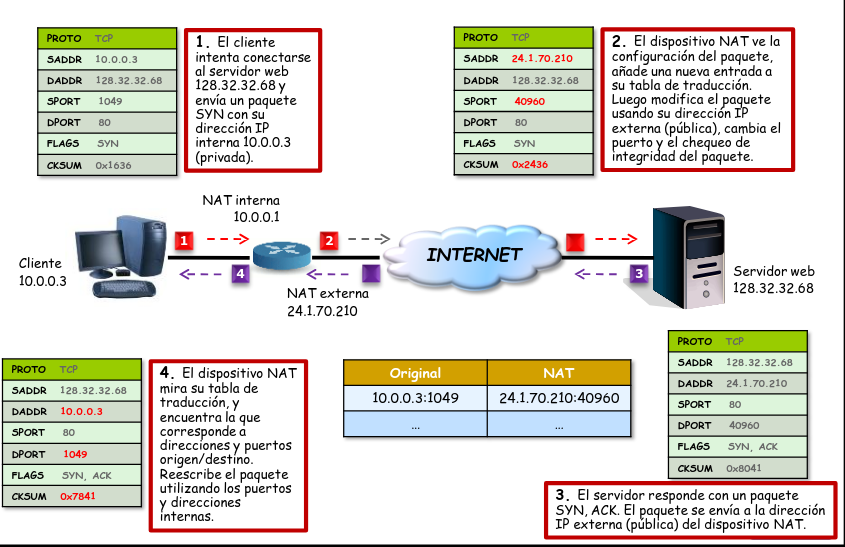
\includegraphics[width=1\textwidth]{images/ProtocoloIp.png}
\end{figure}

\subsubsection{Ejercicio de Asignar Direcciones}

\subsubsection*{Enunciado}
Vamos a suponer que tenemos redes corporativas con 30 dispositivos, direcciones privadas 192.168.0.0, y subred de acceso: dirección pública (ISP)

\subsubsection*{Resolución}

\begin{itemize}
    \item Red 1:
    \begin{itemize}
        \item 30 dispositivos (suponemos que tenemos el router incluido, si no debemos de añadir una dirección para el router)
        \item 30 + 1 dirección de red + 1 dirección de broadcast/difusión = 32 direcciones
        \item 32 = \(2^5\), por lo que necesitamos 5 bits para la subred(para cada equipo) 
        \item Máscara de red: 32 bits - 5 bits = 27 bits = /27
        \item 192.168.0.0/27
        \begin{itemize}
            \item red: \textbf{192.168.0.0}
            \item broadcast: 192.168.0.31
        \end{itemize}
    \end{itemize}
    \item Red 2: \textbf{192.168.0.32}
    \item Red 3: \textbf{192.168.0.65}
\end{itemize}

\begin{tcolorbox}[colback=blue!5!white,colframe=blue!75!black,title=Pregunta de Examen]
    ¿Se puede varios servidores en un mismo punto en la zona privada?
    Sí, sin problema, porque lo que debe de ser distinto es el puerto externo.
    
\end{tcolorbox}

\subsubsection{Encaminamiento}

Se tratade encontrar el mejor camino para transportar paquetes desde un origen a un destino. Se decide paquete a paquete y salto a salto en función de la IP destino del paquete y de las tablas de encaminamiento de cada uno de los routers.

\subsubsection*{Retransmisión salto a salto}
Se puede hacer mediante la resolución local del camino o en el dispositivo origen y todos los intermediarios.

\subsubsection*{Modos de encaminamiento}
\begin{itemize}
    \item Directo: se conoce la dirección IP destino y se envía directamente.
    \item No Directo: se envía a un router que se encargará de enviarlo al destino.
\end{itemize}

\textbf{Nota:} Un router suele estar en varias redes distintas, mientras que un host solo está en una red. En caso de que hay un error a la hora de diriguir debido a la tabla de encamiento, se elige a ruta con máscara más larga.\\

Si no hay fragmentación ni traducción de direcciones (NAT), el datagrama IP no se modifica a lo largo de su recorrido (excepto por campos como el \textit{TTL}, las opciones y el campo de comprobación). A continuación, se describe el proceso de encaminamiento salto a salto para cada datagrama IP:

\paragraph{Proceso de Encaminamiento}
\begin{itemize}
    \item Se extrae la dirección de destino (\texttt{IP\_DESTINO}) del datagrama.
    \item Por cada entrada \( i \) (\( i = 1, \dots, N \)) en la tabla de encaminamiento del nodo, se calcula:
    \[
    \texttt{IPi} = \texttt{IP\_DESTINO} \, \text{AND} \, \texttt{MASCARA\_i}.
    \]
    \item Se verifica si \texttt{IPi} coincide con el identificador de destino (\texttt{Di}):
    \begin{itemize}
        \item Si hay coincidencia y se trata de un \textbf{routing directo}, el datagrama se envía al destino final a través de la interfaz \( i \).
        \item Si hay coincidencia pero no es un \textbf{routing directo}, el datagrama se envía al siguiente salto (\textit{next hop}) a través de la interfaz \( i \).
    \end{itemize}
    \item Si hay varias coincidencias, se selecciona la entrada con la máscara más larga (más específica).
    \item Si no hay coincidencias tras revisar toda la tabla, se genera un error, y es posible que se envíe un mensaje ICMP al origen del datagrama.
\end{itemize}

\paragraph{Encapsulación del Datagrama}
Para encapsular el datagrama en una trama física correspondiente (por ejemplo, Ethernet), se debe consultar la tabla ARP (\textit{Address Resolution Protocol}) para obtener la dirección física del siguiente salto:
\begin{itemize}
    \item Si la dirección física está disponible en la tabla ARP, se utiliza directamente.
    \item Si no se conoce la dirección física, se envía un mensaje de \textbf{broadcast ARP} solicitando la dirección física asociada a la dirección IP destino del enlace.
\end{itemize}

\paragraph{Resumen del Proceso}
El encaminamiento en un nodo IP involucra:
\begin{enumerate}
    \item Determinar la interfaz de salida en función de la tabla de encaminamiento.
    \item Encapsular el datagrama en una trama física usando ARP si es necesario.
    \item Reenviar el datagrama al destino final (en routing directo) o al siguiente salto (en routing indirecto).
\end{enumerate}
Este proceso se repite en cada nodo intermedio hasta que el datagrama llega a su destino final.

\subsubsection*{Comparación de Dirección de Destino y máscara}

Para adivinar que dirección de destino se va a utilizar, se compara la dirección de destino and máscara con la dirección de la tabla de encaminamiento. Si la dirección de destino es igual a la dirección de la tabla de encaminamiento, se envía directamente, si no, se envía al siguiente salto. \textit{Si hay más de una coincidencia(colisión) se elige la entrada de máscara más restrictiva.}

\subsubsection*{Problemas de la tabla de encaminamiento}

Pueden presentar varios problemas como no direccionar algunos tipos de redes, como Internet y demás. Además, es recomendable usar la entrada por defecto que es la que posee la máscara \texttt{0.0.0.0}.

\subsubsection*{Ejercicio: Diseñar la tabla de encaminamiento de un router}

En este caso vamos a diseñar la de R2:
\begin{figure}[H]
    \centering
    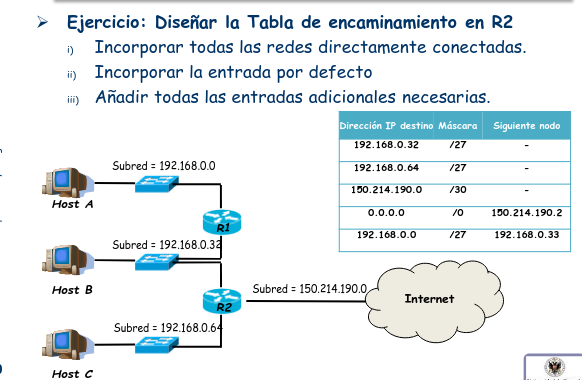
\includegraphics[width=1\textwidth]{images/ejercicioDireR2.png}
\end{figure}
Como podemos ver en esta imagen se trata de asignar en primer lugar las que están más cercanas con una máscara adecuada, luego la del internet, que como dirección de destino usamos la de por defecto ya que no sabemos cómo llegar a ella, y por último la red a la cual tenemos que poner como dirección de destino la más cercana a la red de destino, haciendo de esta manera que el switch haga su función.

\subsection*{Ejercicio}

\subsubsection*{Enunciado}

Imagine una situación donde hay cinco routers RA-RE, RA, RB y RC se conectan cada uno a una red local A, B y C, siendo cada router única puerta de enlace de cada red. RA, RB y RD están conectados entre sí a través de un switch. RC, RD y RE están conectados entre sí a través de un switch. RE conecta a Internet a través de la puerta de acceso especificada por el ISP. Especifique tablas de encaminamiento en los routers. Asigne a voluntad las direcciones IP e interfaces necesarias.

\begin{figure}[H]
    \centering
    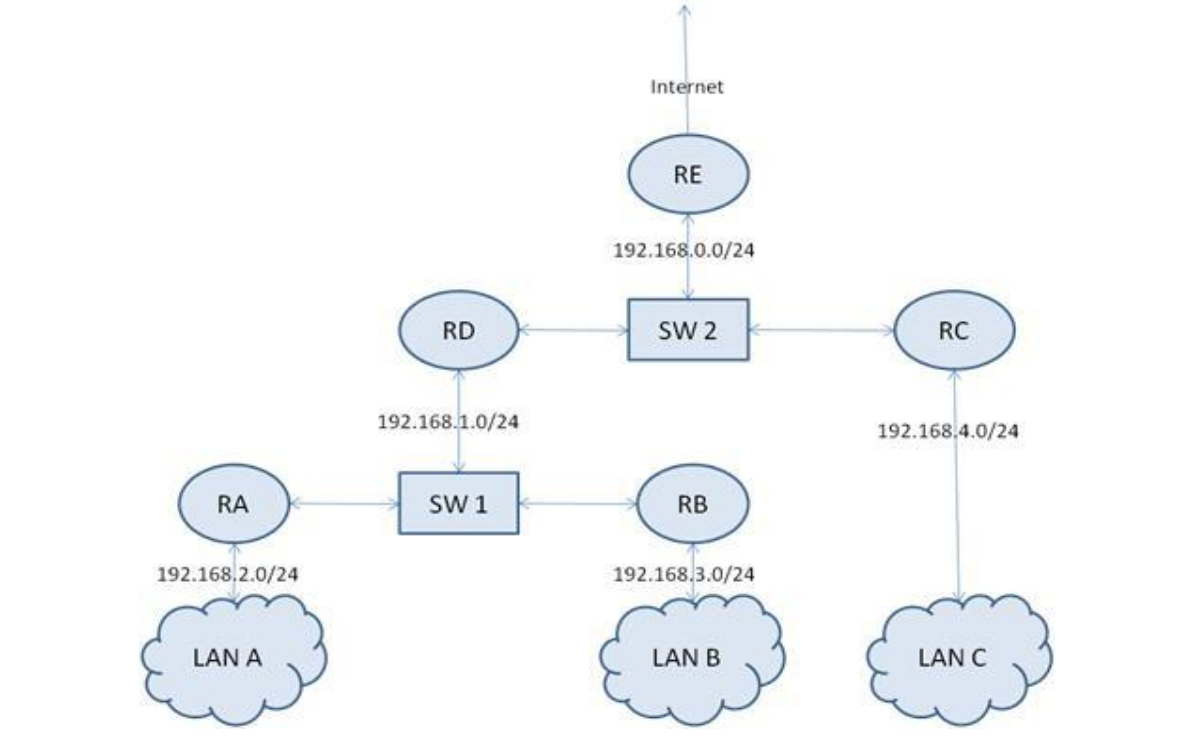
\includegraphics[width=0.9\textwidth]{images/ejercicio_routers.png}
    \caption{Diagrama de Red}
\end{figure}

\subsubsection*{Solución}

Asignaremos direcciones IP e interfaces para cada red y router. Luego, especificaremos las tablas de encaminamiento necesarias para cada router.

\textbf{Direcciones asignadas:}
\begin{itemize}
    \item Red A: 192.168.1.0/24 (RA conectado en interfaz \texttt{fa0/0})
    \item Red B: 192.168.2.0/24 (RB conectado en interfaz \texttt{fa0/0})
    \item Red C: 192.168.3.0/24 (RC conectado en interfaz \texttt{fa0/0})
    \item Conexión RA-RB-RD: 192.168.4.0/24
    \item Conexión RC-RD-RE: 192.168.5.0/24
    \item Conexión RE-ISP: 203.0.113.0/24
\end{itemize}

\textbf{Tablas de encaminamiento:}

\textit{Router RA:}
\begin{tabular}{|c|c|c|c|}
\hline
Red Destino & Máscara & Puerta de Enlace & Interfaz \\
\hline
192.168.2.0 & 255.255.255.0 & 192.168.4.2 & \texttt{fa0/1} \\
192.168.3.0 & 255.255.255.0 & 192.168.4.3 & \texttt{fa0/1} \\
203.0.113.0 & 255.255.255.0 & 192.168.4.3 & \texttt{fa0/1} \\
\hline
\end{tabular}

\textit{Router RB:}
\begin{tabular}{|c|c|c|c|}
\hline
Red Destino & Máscara & Puerta de Enlace & Interfaz \\
\hline
192.168.1.0 & 255.255.255.0 & 192.168.4.1 & \texttt{fa0/1} \\
192.168.3.0 & 255.255.255.0 & 192.168.4.3 & \texttt{fa0/1} \\
203.0.113.0 & 255.255.255.0 & 192.168.4.3 & \texttt{fa0/1} \\
\hline
\end{tabular}

\textit{Router RC:}
\begin{tabular}{|c|c|c|c|}
\hline
Red Destino & Máscara & Puerta de Enlace & Interfaz \\
\hline
192.168.1.0 & 255.255.255.0 & 192.168.5.2 & \texttt{fa0/1} \\
192.168.2.0 & 255.255.255.0 & 192.168.5.2 & \texttt{fa0/1} \\
203.0.113.0 & 255.255.255.0 & 192.168.5.3 & \texttt{fa0/1} \\
\hline
\end{tabular}

\textit{Router RD:}
\begin{tabular}{|c|c|c|c|}
\hline
Red Destino & Máscara & Puerta de Enlace & Interfaz \\
\hline
192.168.1.0 & 255.255.255.0 & 192.168.4.1 & \texttt{fa0/0} \\
192.168.2.0 & 255.255.255.0 & 192.168.4.2 & \texttt{fa0/0} \\
192.168.3.0 & 255.255.255.0 & 192.168.5.1 & \texttt{fa0/1} \\
203.0.113.0 & 255.255.255.0 & 192.168.5.3 & \texttt{fa0/1} \\
\hline
\end{tabular}

\textit{Router RE:}
\begin{tabular}{|c|c|c|c|}
\hline
Red Destino & Máscara & Puerta de Enlace & Interfaz \\
\hline
192.168.1.0 & 255.255.255.0 & 192.168.5.1 & \texttt{fa0/0} \\
192.168.2.0 & 255.255.255.0 & 192.168.5.1 & \texttt{fa0/0} \\
192.168.3.0 & 255.255.255.0 & 192.168.5.1 & \texttt{fa0/0} \\
\hline
\end{tabular}

Esto asegura que cada router pueda alcanzar las demás redes y enrutar tráfico hacia Internet a través de RE.


\subsubsection*{Aumento de escalabilidad y de administración}

Internet se jerarquiza mediante Sistemas Autónomos(SA). Un SA es un conjunto de redes y de routers que son gestionados por una autoridad. Cada uno informa a otros SA de las redes accesibles, existen un router responsable de ello, llamado router exterior. Cada uno de los SA se identifica mediante un entero de 16 bits \textbf{pero, desde 2007 es de 32 bits}.


\subsubsection*{Niveles de Encaminamiento}

\begin{itemize}
    \item \textbf{Algoritmos IGP (Interior Gateway Protocol):}
        \begin{itemize}
            \item Se utilizan dentro de un Sistema Autónomo (SA) para el encaminamiento de paquetes.
            \item Los administradores de red tienen libertad para elegir el protocolo que mejor se adapte a sus necesidades.
            \item Ejemplos comunes incluyen:
                \begin{itemize}
                    \item \textbf{OSPF (Open Shortest Path First):} Un protocolo de estado de enlace que utiliza el algoritmo de Dijkstra para calcular la ruta más corta.
                    \item \textbf{RIP (Routing Information Protocol):} Un protocolo de vector de distancia que utiliza el número de saltos como métrica.
                    \item \textbf{EIGRP (Enhanced Interior Gateway Routing Protocol):} Un protocolo híbrido desarrollado por Cisco que combina características de los protocolos de vector de distancia y de estado de enlace.
                \end{itemize}
        \end{itemize}

    \item \textbf{Algoritmos EGP (Exterior Gateway Protocol):}
        \begin{itemize}
            \item Se utilizan para el encaminamiento de paquetes entre diferentes Sistemas Autónomos (SA).
            \item En Internet, existe una norma única para el encaminamiento entre SA, que es el protocolo BGP.
            \item \textbf{BGP (Border Gateway Protocol):} 
                \begin{itemize}
                    \item Es el protocolo estándar utilizado para el intercambio de información de encaminamiento entre Sistemas Autónomos.
                    \item Utiliza una tabla de encaminamiento para mantener la información de las rutas disponibles y toma decisiones basadas en políticas configuradas por los administradores de red.
                    \item BGP es un protocolo de vector de ruta que considera múltiples atributos para determinar la mejor ruta.
                \end{itemize}
        \end{itemize}
\end{itemize}

\subsubsection*{Diferentes protocolos}

\begin{itemize}
    \item RIP (Routing Information Protocol)
    \subsubsection*{RIP (“Routing Information Protocol” RFC 1058, 2453, 4822)}

    \begin{itemize}
        \item \textbf{Protocolo de la capa de aplicación:} Opera sobre UDP, puerto 520.
        \item \textbf{Algoritmo:} Vector-distancia (métrica basada en el número de saltos).
        \item \textbf{Funcionamiento:}
        \begin{itemize}
            \item Periódicamente (por defecto cada 30 segundos), cada router RIP recibe de todos sus vecinos (usando la dirección multicast \texttt{224.0.0.9}) los vectores-distancia para todos los posibles destinos.
            \item Para cada destino, se selecciona como siguiente salto el vecino que anuncie el menor coste. La métrica para ese destino se actualiza sumando uno al coste anunciado.
        \end{itemize}
        \item \textbf{Problemas:}
        \begin{itemize}
            \item \textbf{Convergencia lenta:} Las malas noticias tardan en propagarse.
            \item \textbf{“Cuenta al infinito”:} Los costos pueden incrementarse indefinidamente.
        \end{itemize}
        \item \textbf{Soluciones:}
        \begin{itemize}
            \item Split horizon.
            \item Hold down.
            \item Poison reverse.
        \end{itemize}
        \item \textbf{Comando útil:} Para más detalles, consultar el manual del comando \texttt{routed} en sistemas Linux (\texttt{man routed}).
    \end{itemize}

    \item OSPF 
    \subsubsection*{OSPF (RFC 2328)}

    \begin{itemize}
        \item Basado en estado del enlace (\textit{link state}), donde el coste es proporcional a \(1 / \text{velocidad del enlace}\).
        \item Permite rutas alternativas y balanceo de carga.
        \item Gestión en base a áreas independientes.
        \item Minimiza difusión mediante routers designados (\textit{Designated Routers, DR}).
        \item Mensajes utilizados:
        \begin{itemize}
            \item Hello.
            \item Database description.
            \item Link status request, update y acknowledgment.
        \end{itemize}
    \end{itemize}

    Enlace de imagen: \url{https://i0.wp.com/theosnews.com/wp-content/uploads/2015/05/2-Configuraci%C3%B3n-de-OSPF-Redes-directamente-conectadas.jpg?ssl=1}

\end{itemize}



\begin{tcolorbox}[colback=blue!5!white,colframe=blue!75!black,title=Pregunta de Examen]
    \textbf{Si R1 quiere ir a R3 por dos caminos con el mismo número de saltos pero con A=100Mbps y B=10Mbps,¿Cuál cojo?}
    Solo cojo un camino si mejora el primero que me dan.
\end{tcolorbox}

\subsubsection{Formato del Datagrama}

Imagen: pincha \href{https://blogger.googleusercontent.com/img/b/R29vZ2xl/AVvXsEiEEYTrMsBMcUuMgs5GyGPSG0T5O2QECfeWvZaik5PAOFnwYuSL3oMsYZKoTSd4F8kEhdOBzseuzHFQyWU4F22N2D7eWP_JwpUukMVGNcF5EbRSWdFb2B0qndVeLgDerXWbrSH79YsKmlA/w1200-h630-p-k-no-nu/Datagrama+IP.+IP+Datagram.jpg}{aquí}.



\subsubsection{Fragmentación IPv4}

La fragmentación en IPv4 es un mecanismo que permite dividir un datagrama en fragmentos más pequeños para que puedan adaptarse al tamaño máximo permitido por la Unidad Máxima de Transferencia (\textit{MTU}) de las subredes por las que pasa. A continuación, se explican los aspectos más relevantes:

\begin{itemize}
    \item \textbf{Tamaño máximo del datagrama:} El tamaño máximo permitido para un datagrama IPv4 es de 65535 bytes (\(2^{16} - 1\)), incluyendo el encabezado y los datos.
    \item \textbf{Adaptación a la MTU:} Cada enlace en una red puede tener una MTU diferente. Si el tamaño de un datagrama excede la MTU de una subred, debe ser fragmentado para poder ser transmitido.
    \item \textbf{Ensamblado en el destino final:} Los fragmentos de un datagrama solo pueden ser ensamblados en el destino final. Los nodos intermedios no realizan ensamblado, lo que evita complejidad adicional en el encaminamiento.
    \item \textbf{Desplazamiento (\textit{offset}):} Cada fragmento incluye un campo que indica su posición relativa dentro del datagrama original. Esto permite que los fragmentos se ensamblen correctamente en el destino final.
    \item \textbf{Indicadores de control:}
    \begin{itemize}
        \item \textbf{Don't Fragment (DF):} Si este indicador está activado, el datagrama no puede ser fragmentado. Si el datagrama excede la MTU, se descarta y se envía un mensaje ICMP al origen.
        \item \textbf{More Fragments (MF):} Este indicador se activa para todos los fragmentos excepto el último, indicando que el datagrama original está dividido en partes.
    \end{itemize}
\end{itemize}

\paragraph{Ejemplo de Fragmentación}

Supongamos un datagrama con un tamaño total de 4000 bytes que necesita ser transmitido a través de una subred con una MTU de 1500 bytes. La fragmentación se realiza de la siguiente manera:
\begin{itemize}
    \item El encabezado IP ocupa 20 bytes, dejando 1480 bytes para los datos en cada fragmento.
    \item Se generan los siguientes fragmentos:
    \begin{itemize}
        \item \textbf{Fragmento 1:} Datos del byte 0 al byte 1479 (\texttt{offset = 0}).
        \item \textbf{Fragmento 2:} Datos del byte 1480 al byte 2959 (\texttt{offset = 185}, ya que cada unidad de \textit{offset} corresponde a 8 bytes).
        \item \textbf{Fragmento 3:} Datos del byte 2960 al byte 3999 (\texttt{offset = 370}, último fragmento con \texttt{MF = 0}).
    \end{itemize}
\end{itemize}

Para profundizar en el tema de offset picha \href{https://github.com/ElblogdeIsmael/ElblogdeIsmael.github.io/blob/main/Asignaturas/Tercer%20A%C3%B1o/FR/Resumenes/ETSIIT/offset.md}{aquí.}

\paragraph{Ventajas y Desventajas de la Fragmentación}
\begin{itemize}
    \item \textbf{Ventajas:} Permite la transmisión de datagramas grandes a través de redes con diferentes MTUs.
    \item \textbf{Desventajas:} Introduce sobrecarga adicional en términos de encabezados y complica el ensamblado en el destino. Además, si un fragmento se pierde, el datagrama completo debe ser retransmitido.
\end{itemize}


\subsubsection{Ejercicio Típico de Examen sobre la fragmentacion IPv4}


\begin{figure}[H]
    \centering
    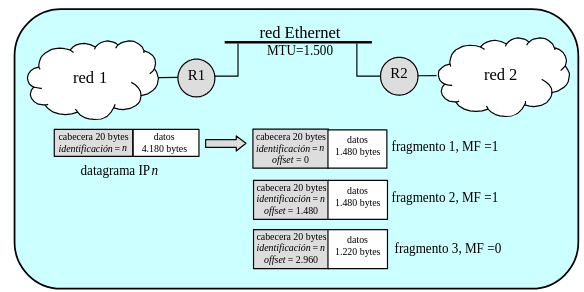
\includegraphics[width=1\textwidth]{images/fragIPV4.png}
\end{figure}

\subsubsection*{Comentarios del Ejercicio}

Para la realización del ejercicio debemos de seguir los siguientes pasos y repetirlos hasta que no se necesiten más fragmentos, es decir, hasta que el MF = 0. Debemos de tener en cuenta que la cabecera ocupa siempre 20 bytes, por lo tanto, si nuestro MTU es 1500, solo podremos transportar el paquete en unidades de 1480 bytes, siendo esto el valor máximo. El offset mide el desplazamiento del paquete, en otras palabras, la suma total de los bytes que se han transmitido.


\subsubsection{Diferencias entre IPv4 y IPv6}


\begin{table}[H]
    \centering
    \begin{tabular}{|p{4cm}|p{4cm}|p{7cm}|}
    \hline
    \textbf{Característica} & \textbf{IPv4} & \textbf{IPv6} \\ \hline
    Longitud de la dirección & 32 bits & 128 bits \\ \hline
    Espacio de direcciones & \textasciitilde 4.3 mil millones & 340 undecillones (casi ilimitado) \\ \hline
    Formato & Decimal (ej. 192.168.0.1) & Hexadecimal (ej. 2001:0db8:8a2e:0370:7334) \\ \hline
    Configuración & Manual o DHCP & Autoconfiguración sin estado (SLAAC) \\ \hline
    Seguridad & Opcional (IPsec) & IPsec obligatorio \\ \hline
    Fragmentación & Los routers pueden fragmentar & Solo el dispositivo emisor fragmenta \\ \hline
    Encabezado de paquetes & Complejo y variable & Simplificado y fijo \\ \hline
    QoS & Limitado (TOS) & Optimizado (Flow Label) \\ \hline
    Compatibilidad & Amplia, pero limitado por direcciones & No compatible directamente con IPv4 \\ \hline
    Optimización para móviles & Menos eficiente & Mejor rendimiento en redes móviles \\ \hline
    \end{tabular}
\end{table}

\subsubsection*{Tabla comentada}

\begin{itemize}
    \item \textbf{Longitud de la dirección:}
    \begin{itemize}
        \item IPv4 utiliza direcciones de 32 bits, lo que limita el espacio de direcciones disponibles.
        \item IPv6 expande las direcciones a 128 bits, proporcionando un espacio de direccionamiento prácticamente ilimitado.
    \end{itemize}

    \item \textbf{Espacio de direcciones:}
    \begin{itemize}
        \item IPv4 puede manejar aproximadamente 4.3 mil millones de direcciones únicas, un recurso que ya se ha agotado en gran medida.
        \item IPv6 proporciona \( 340 \) undecillones de direcciones, suficientes para las necesidades actuales y futuras.
    \end{itemize}

    \item \textbf{Formato:}
    \begin{itemize}
        \item IPv4 utiliza un formato decimal, como \texttt{192.168.0.1}.
        \item IPv6 adopta un formato hexadecimal, más eficiente para expresar direcciones largas, como \texttt{2001:0db8:8a2e:0370:7334}.
    \end{itemize}

    \item \textbf{Configuración:}
    \begin{itemize}
        \item IPv4 requiere configuración manual o el uso de DHCP.
        \item IPv6 ofrece autoconfiguración sin estado mediante SLAAC, simplificando la gestión de redes.
    \end{itemize}

    \item \textbf{Seguridad:}
    \begin{itemize}
        \item IPv4 soporta IPsec de forma opcional.
        \item IPv6 integra IPsec de manera obligatoria, mejorando la seguridad por defecto.
    \end{itemize}

    \item \textbf{Fragmentación:}
    \begin{itemize}
        \item En IPv4, los routers pueden fragmentar los paquetes.
        \item En IPv6, la fragmentación solo se realiza en el dispositivo emisor, mejorando la eficiencia del encaminamiento.
    \end{itemize}

    \item \textbf{Encabezado de paquetes:}
    \begin{itemize}
        \item IPv4 tiene un encabezado complejo y variable, lo que puede aumentar la latencia.
        \item IPv6 utiliza un encabezado simplificado y fijo, optimizando el procesamiento en los nodos.
    \end{itemize}

    \item \textbf{Calidad de servicio (QoS):}
    \begin{itemize}
        \item IPv4 ofrece un soporte limitado mediante el campo TOS (\textit{Type of Service}).
        \item IPv6 mejora la QoS mediante etiquetas de flujo (\textit{Flow Label}), proporcionando mayor granularidad.
    \end{itemize}

    \item \textbf{Compatibilidad:}
    \begin{itemize}
        \item IPv4 es ampliamente compatible con sistemas y dispositivos existentes.
        \item IPv6 no es directamente compatible con IPv4, lo que requiere mecanismos de transición como túneles o direcciones mixtas.
    \end{itemize}

    \item \textbf{Optimización para móviles:}
    \begin{itemize}
        \item IPv4 es menos eficiente en redes móviles.
        \item IPv6 está diseñado para mejorar el rendimiento en estas redes, adaptándose a las necesidades modernas.
    \end{itemize}
\end{itemize}


    

\subsection{Asociación de la capa de enlace: protocolo ARP}


\subsubsection{Direcciones MAC}

Las direcciones \textbf{MAC (Medium Access Control)} son identificadores únicos que se utilizan para direccionar paquetes a nivel de la capa de enlace en redes Ethernet (cableadas) y WiFi. Estas direcciones juegan un papel clave en el encaminamiento de datos dentro de una red local.

\paragraph{Uso de las Direcciones MAC}

Una vez que se realiza la redirección a nivel de IP, el paquete debe ser enviado a la dirección MAC del siguiente nodo en la ruta hacia el destino final. Este proceso asegura que los datos lleguen al nodo correcto dentro de la red local antes de ser enviados a la siguiente etapa.

\paragraph{Formato de las Direcciones MAC}

Las direcciones MAC tienen un formato estándar de 6 bytes (48 bits) representados en notación hexadecimal y separados por guiones:
\[
\texttt{HH-HH-HH-HH-HH-HH}
\]
Por ejemplo:
\[
\texttt{00-24-21-A8-F7-6A}
\]

\paragraph{Asignación de Direcciones MAC}

\begin{itemize}
    \item Cada dirección MAC es única y está asignada por la \textbf{IEEE (Institute of Electrical and Electronics Engineers)}.
    \item Las direcciones se asignan en lotes de \(2^{24}\) direcciones para cada fabricante de dispositivos de red.
\end{itemize}

\paragraph{Dirección de Difusión (Broadcast)}

En las redes locales, la dirección \textbf{FF-FF-FF-FF-FF-FF} se utiliza para enviar paquetes a todos los dispositivos conectados en la red. Esto es útil para realizar descubrimientos, como en el caso del protocolo ARP (Address Resolution Protocol).

Para ver el formato ARP accede al siguiente enlace: \url{https://i.ytimg.com/vi/qJZzX0V8Opg/maxresdefault.jpg}

\paragraph{Resumen}

Las direcciones MAC son esenciales para la comunicación dentro de redes locales, permitiendo la identificación única de dispositivos y facilitando tanto la comunicación unicast (entre dos nodos específicos) como la difusión a todos los nodos de la red.



\subsection{El Protocolo ICMP}

El \textbf{ICMP (Internet Control Message Protocol)} es un protocolo de la capa de red utilizado para gestionar y reportar situaciones de error o eventos relacionados con el funcionamiento de IP. Se clasifica como un protocolo de señalización, ya que no transporta datos de usuario, sino información sobre el estado de la red.

\subsubsection*{Características del Protocolo ICMP}

\begin{itemize}
    \item \textbf{Propósito:} ICMP se utiliza para informar sobre errores en el funcionamiento de IP y para facilitar diagnósticos de red.
    \item \textbf{Dirección del mensaje:} Los mensajes ICMP suelen enviarse hacia el origen del datagrama IP que generó el evento, excepto en casos como solicitudes de eco (\textit{ping}).
    \item \textbf{Encapsulación:} Los mensajes ICMP se encapsulan dentro de paquetes IP para su transmisión.
    \item \textbf{Cabecera:} La cabecera ICMP tiene un tamaño fijo de 32 bits y contiene la siguiente información:
    \begin{itemize}
        \item \textbf{Tipo (8 bits):} Indica el tipo de mensaje ICMP.
        \item \textbf{Código (8 bits):} Especifica el subtipo del mensaje, proporcionando mayor detalle.
        \item \textbf{Comprobación (16 bits):} Un campo para la detección de errores en el mensaje ICMP.
    \end{itemize}
    \item \textbf{Incluye información del datagrama original:} El mensaje ICMP incluye la cabecera del datagrama IP que disparó el evento, para que el origen pueda identificar el problema.
\end{itemize}

\subsubsection*{Tipos Comunes de Mensajes ICMP}

\begin{itemize}
    \item \textbf{Destino inalcanzable:} Informa al origen que un datagrama no pudo ser entregado.
    \item \textbf{Tiempo excedido:} Indica que un datagrama ha sido descartado porque excedió su tiempo de vida (\textit{Time-to-Live, TTL}).
    \item \textbf{Redirección:} Notifica a un host que debe utilizar otra ruta para alcanzar un destino.
    \item \textbf{Solicitud y respuesta de eco (\textit{Ping}):} Se utiliza para comprobar la conectividad y medir el tiempo de respuesta entre dos dispositivos.
\end{itemize}

\subsubsection*{Resumen}

El protocolo ICMP es una herramienta esencial para la gestión de redes IP. Al proporcionar información sobre errores y diagnósticos, permite mantener la integridad y el rendimiento de la comunicación en la red. Aunque no transporta datos de usuario, su papel en la señalización lo convierte en un componente fundamental de la capa de red.


Para ver los mensajes ICMP, accede a este enlace: \url{https://w3.ual.es/~vruiz/Docencia/Apuntes/Networking/Protocols/Level-3/04-ICMP/mensajes_ICMP.png}







\subsection{DHCP: Autoconfiguración de la capa de red}


El \textbf{DHCP (Dynamic Host Configuration Protocol)} es un protocolo de red que permite a los dispositivos obtener automáticamente configuraciones esenciales para su conexión en una red IP. Es ampliamente utilizado para asignar dinámicamente direcciones IP, así como otros parámetros de configuración de red.

\subsubsection*{Funcionamiento del DHCP}

El protocolo DHCP sigue un modelo cliente-servidor en el que los clientes solicitan información de configuración y el servidor responde con los datos necesarios. El proceso se compone de cuatro etapas principales:
\begin{enumerate}
    \item \textbf{Discover:} El cliente envía un mensaje de difusión DHCP Discover buscando servidores DHCP disponibles en la red.
    \item \textbf{Offer:} El servidor responde con un mensaje DHCP Offer, que incluye una dirección IP disponible y otros parámetros.
    \item \textbf{Request:} El cliente envía un mensaje DHCP Request indicando su intención de usar la dirección IP ofrecida.
    \item \textbf{Acknowledge:} El servidor confirma la asignación con un mensaje DHCP Acknowledge, y el cliente puede comenzar a usar la dirección IP.
\end{enumerate}

\subsubsection*{Parámetros Configurados por DHCP}

El servidor DHCP no solo asigna direcciones IP, sino que también puede proporcionar otros parámetros de configuración importantes, tales como:
\begin{itemize}
    \item Máscara de subred.
    \item Puerta de enlace predeterminada (\textit{default gateway}).
    \item Servidores DNS.
    \item Tiempo de arrendamiento (\textit{lease time}) para la dirección IP asignada.
    \item Opciones específicas de la red, como rutas estáticas.
\end{itemize}

\subsubsection*{Ventajas del DHCP}

\begin{itemize}
    \item \textbf{Automatización:} Reduce la necesidad de configurar manualmente cada dispositivo en la red.
    \item \textbf{Eficiencia:} Permite reutilizar direcciones IP, lo que es especialmente útil en redes con un número limitado de direcciones disponibles.
    \item \textbf{Facilidad de gestión:} Centraliza la administración de la configuración de red.
\end{itemize}

\subsubsection*{Desventajas del DHCP}

\begin{itemize}
    \item \textbf{Dependencia del servidor:} Si el servidor DHCP falla, los nuevos dispositivos no podrán obtener configuración de red.
    \item \textbf{Falta de control fijo:} Aunque es posible asignar direcciones fijas, DHCP está diseñado principalmente para asignaciones dinámicas.
\end{itemize}

\subsubsection*{Ejemplo de Funcionamiento}

Proceso de una sesión DHCP entre cliente y servidor: \url{https://blogger.googleusercontent.com/img/b/R29vZ2xl/AVvXsEhyvPCPxrYJdM7ra-zKKv-9ptw5el9t7mQUvzKB6GGjV8I07_0URHw1aHtl652Ks0vCRss-PWtPG1BWwn8xnimpH_klN0Eac_Wr6-gvvJzzPccANoflbWWt0KkuT3zidC59Do4A8bCYHDoe/s1600/DHCP_Cliente_Servidor.png}

\subsubsection*{Resumen}

El protocolo DHCP es fundamental para la gestión dinámica y automatizada de redes IP. Su capacidad para asignar y gestionar parámetros de configuración de red de manera eficiente lo convierte en una herramienta esencial en redes modernas, tanto domésticas como empresariales.





%diapos 56 de mi tablet
%https://chatgpt.com/c/67693401-0fdc-8012-8dea-a3b6f3ca0d4a





% \section{Otras definiciones}

% \begin{itemize}
%     \item El programa \textbf{ping} se utiliza para comprobar el estado de un host utilizando el protocolo
%     ICMP. El host origen manda un mensaje de solicitud de eco con un identificador. Si el
%     destino está conectado, la comunicación es posible y está correctamente configurada,
%     el host origen recibirá un mensaje de respuesta de eco con el mismo código. Este
%     programa sirve asimismo para calcular empíricamente la latencia de la conexión.
% \end{itemize}




    

\end{document}
